\documentclass[12pt]{article}
%\usepackage{scicite}
%\usepackage{times}
\usepackage{pdfpages}
\author{Aaron Spring}
%\usepackage[ansinew]{inputenc}
\usepackage{amsmath}
\usepackage{siunitx}
\usepackage[colorlinks=true, urlcolor=blue, linkcolor=darkgray,citecolor=blue]{hyperref}
%\usepackage[german]{babel}
\usepackage{float}
%\usepackage[numbers]{natbib}
\usepackage[authoryear]{natbib}
%\usepackage[pliannatuthoryear]{natbib}
\usepackage{indentfirst}
\usepackage{amsmath}
%\renewcommand{\vec}[1]{\boldsymbol{#1}}

\usepackage{graphicx}
\graphicspath{{/home/mpim/m300524/MSc_Thesis/gfx/}}

% The following parameters seem to provide a reasonable page setup.

\topmargin 0.0cm
\oddsidemargin 0.2cm
\textwidth 16cm 
\textheight 21cm
\footskip 1.0cm

%\newcommand{\memberpositive}{m105_1994_2001}
\newcommand{\memberpositive}{m178_1985_1992} %funktioniert am besten
%\newcommand{\memberpositive}{m182_1988_1995} % zweitbesten


%\newcommand{\membernegative}{m113_1986_1993}
\newcommand{\membernegative}{m143_1995_2002}


%The next command sets up an environment for the abstract to your paper.

%\newenvironment{sciabstract}{%
%\begin{quote} \bf}
%{\end{quote}}


% If your reference list includes text notes as well as references,
% include the following line; otherwise, comment it out.

\renewcommand\refname{References and Notes}

% The following lines set up an environment for the last note in the
% reference list, which commonly includes acknowledgments of funding,
% help, etc.  It's intended for users of BibTeX or the {thebibliography}
% environment.  Users who are hand-coding their references at the end
% using a list environment such as {enumerate} can simply add another
% item at the end, and it will be numbered automatically.

%\newcounter{lastnote}
%\newenvironment{scilastnote}{%
%\setcounter{lastnote}{\value{enumiv}}%
%\addtocounter{lastnote}{+1}%
%\begin{list}%
%{\arabic{lastnote}.}
%{\setlength{\leftmargin}{.22in}}
%{\setlength{\labelsep}{.5em}}}
%{\end{list}}




\begin{document} 

% Double-space the manuscript.

\baselineskip24pt

% Make the title.
\title{Internal variability of the Southern Ocean carbon sink in MPI-ESM large ensemble simulations: \\ assessment of westerly wind changes}

\maketitle 
%\Huge
%\textbf{Outline}

\normalsize
\tableofcontents

\newpage

\section{Introduction}

\paragraph{why Southern Ocean is important} carbon budget oceanic uptake \citep{Sabine2004} \citep{Quere2016a} SO as constraint to reduce model uncertainties \citep{Kessler2016}

\paragraph{Southern Ocean observations and call for models}
Observation-based estimates report a large variability in the Southern Ocean carbon sink \citep{LeQuere2007,landschuetzer2015}. Sparse observational data lack the ability to show the dynamics of internally varying processes, which demands for the evaluation with models.
 
 
%why did Tatiana want me to do this:
%all coupled models fail to reproduce SO variability, ocean-only models with NCEP forcing catch it, so its probably the winds 
 
\paragraph{Hypothesis}
The Southern Annular Mode (SAM), characterizing the strength and position of the westerly winds, is known to be the dominant mode of climate variability in the Southern hemisphere \citep{Thompson2000}.  Supposing the strength and position of the westerlies winds as the major reason for climate variability for the Southern Ocean, how does the carbon system respond? Strengthening westerlies increase upwelling, so more carbon-rich waters entrain the upper ocean and hence outgas. This upwelling also brings additional nutrients for the deep ocean, which might foster primary production. However, if the wind mixes too strong though, primary production decreases because of light limitation \citep{Sverdrup1953} or other physical controls of biological production.

 
%\begin{figure}[h!]
%\centering
%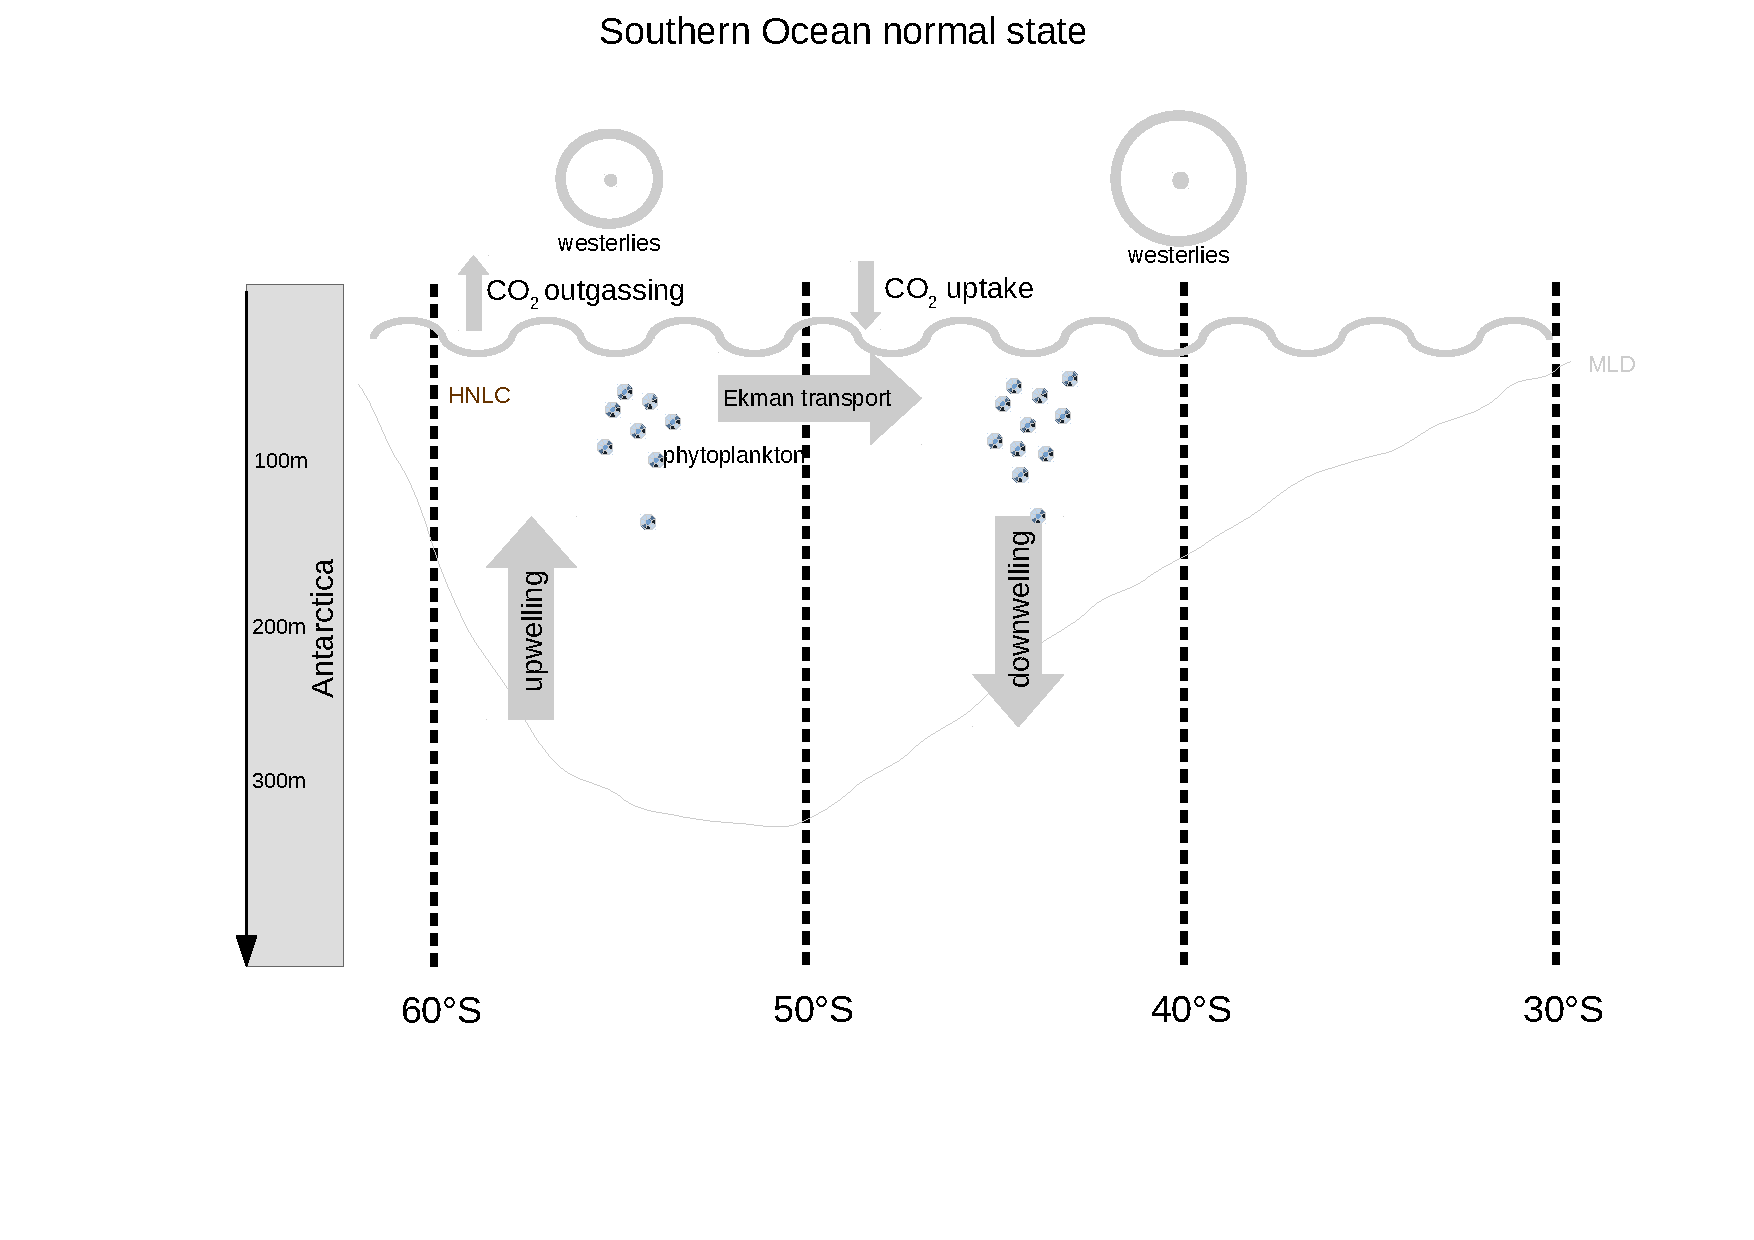
\includegraphics[scale=.5,trim=2cm 3.5cm 2cm 1.8cm,clip,page=1]{SO_schematics}
%\vspace{-3mm}
%\caption{Schematic illustration of the Southern Ocean ; probably wrong location here, but where to put it? Results I after the mean state results?}
%\end{figure}

\paragraph{Previous studies on co2flux mechanism and trends, modelling and observations}
Previous modeling studies were studying the impact of SAM on the carbon sink \citep{Lovenduski2007,Hauck2013} or long-term carbon trends \citep{wang2012} using ocean-only models with atmospheric historic forcing. biology response on SAM \citep{Lovenduski2005}

\paragraph{what's new?}
coupled model for internal variability study: are ensembles able to reproduce decadal trends? CESM ICLE doesnt; Int. Var. co2flux controls in HAMOCC


\paragraph{What I do and research questions}
By using a large ensemble simulation based on the Max-Planck-Institute Earth System Model (MPI-ESM), I investigate the variability of the oceanic carbon uptake. I try to answer the following questions: 
\begin{enumerate}
\item How large is the modeled internal variability of the Southern Ocean carbon sink? 
\item Do I find similar trends to those observed in the 1990s and 2000s in a large ensemble? 
\item How does variability in physical processes influence the carbon sink?

\end{enumerate}

\clearpage

\section{Methods}

\subsection{Model description}

\paragraph{listing MPI-ESM components} The MPI-ESM version 1.1.00p2  \footnote[1]{full source code: \url{https://code.zmaw.de/projects/mpi-esm/repository/show/tags/mpiesm-1.1.00p2}} with a low-resolution configuration (MPI-ESM-LR) is used for the large ensemble simulations \citep{Giorgetta2013}. The atmosphere component ECHAM6.3 runs on a T63 grid, corresponding to 1.9$^\circ$ horizontal resolution, with 47 vertical layers up to 0.01 hPa \citep{Stevens2013}. 
Atmospheric pCO$_2$ levels are prescribed due to the CMIP5 protocol and well mixed \citep{Taylor2012}. The carbon cycle is not coupled, so called diagnostic, so effects of changes in the terrestrial or oceanic carbon sink are not reflected in the atmospheric pCO$_{\text{2,atm}}$. Since there is no biogeochemical riverine exchange, terrestrial and oceanic carbon sink do not interact (Fig. \ref{fig:MPIESM}). The ocean component MPI Ocean Model (MPIOM) has a horizontal resolution of 1.5$^\circ$ on average, relating to a spatial resolution of 150km at 30$^\circ$S and 40km in Antarctic coastal waters, and 40 fixed-depth vertical levels \citep{Jungclaus2013}. The Hamburg Ocean Carbon Cycle Model (HAMOCC) represents the ocean biogeochemistry component and aims to describe the carbon cycle (Fig. \ref{fig:HAMOCC}) \citep{Ilyina2013}.

\begin{figure}[h!]
	\centering 
	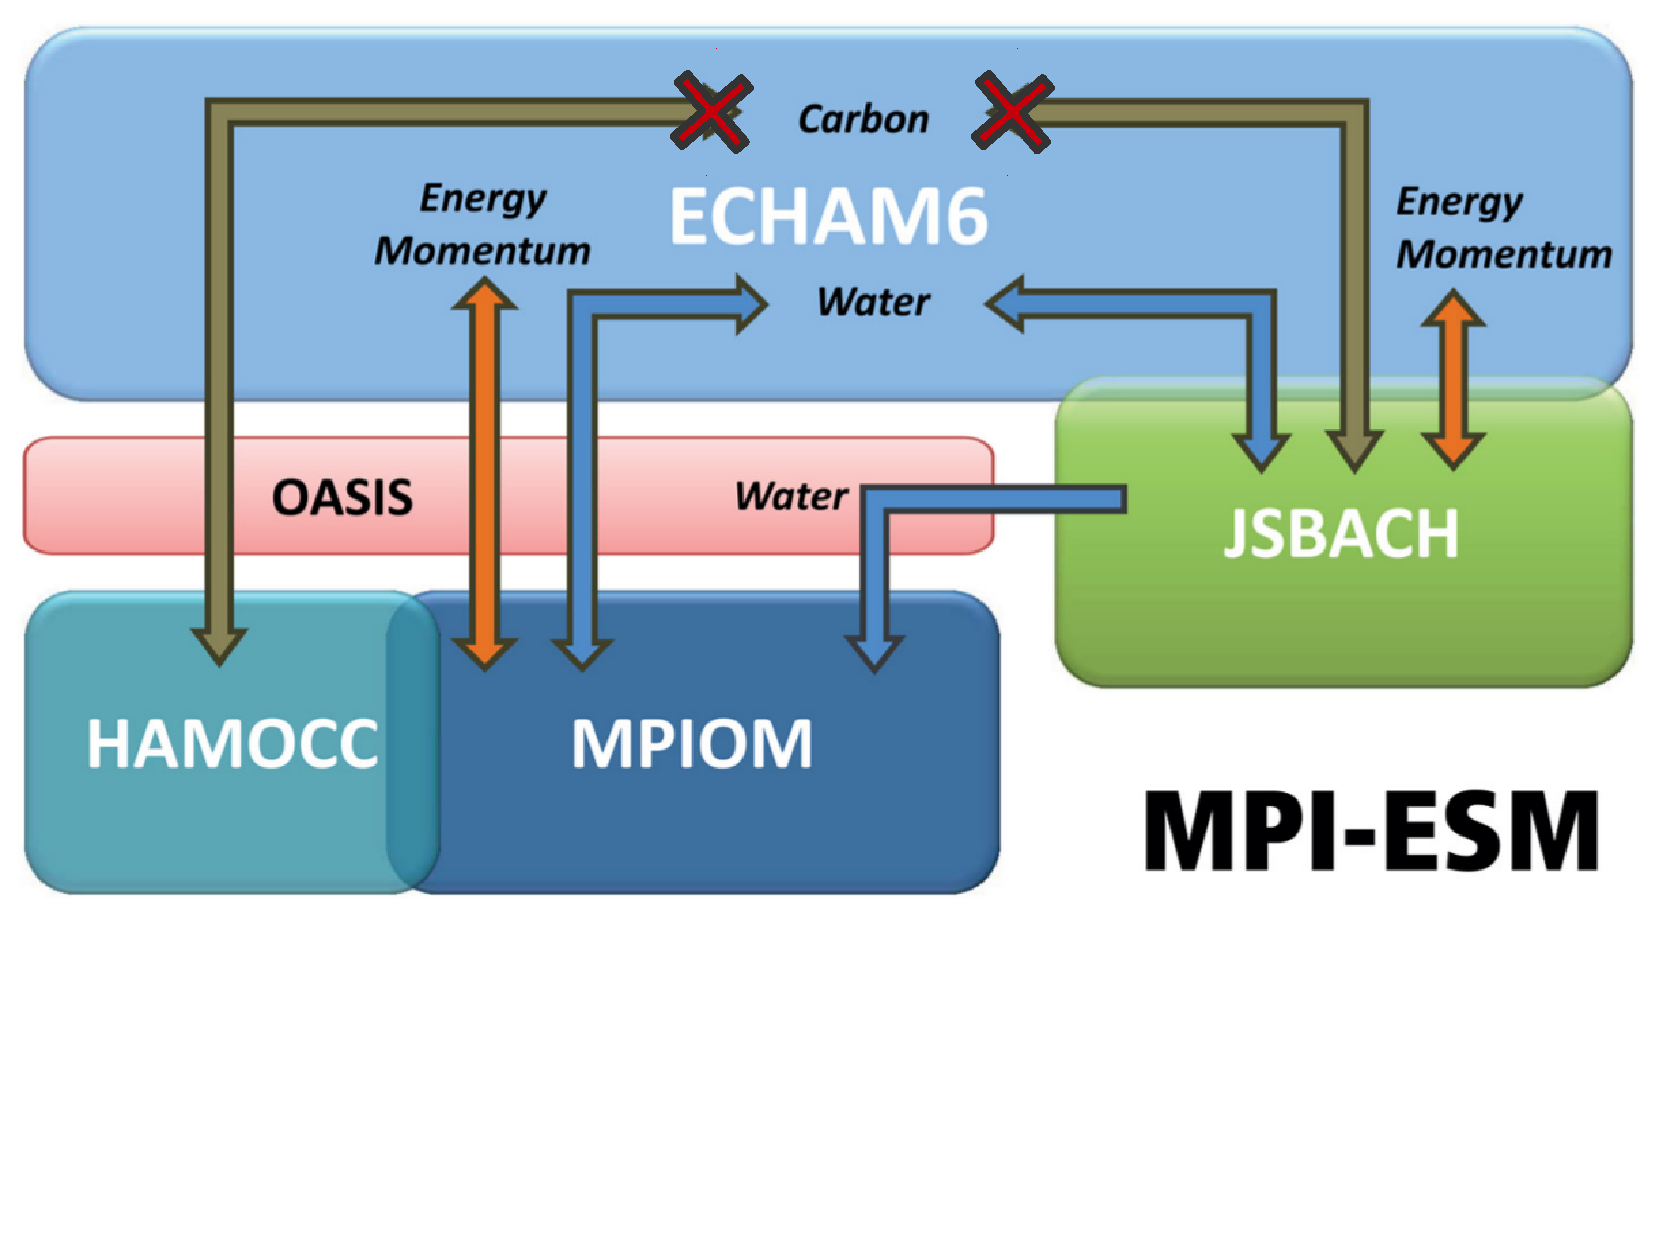
\includegraphics[scale=.5,trim=0cm 5.87cm 0cm 0cm,clip]{MPIESM.pdf}
	\caption{Schematic overview on the different components in MPI-Earth-System-Model with a diagnostic carbon cycle \citep{Giorgetta2013}}
	\label{fig:MPIESM}
\end{figure}

\subsubsection*{I briefly explain how processes affecting the carbon cycle are implemented and subject to internal variability}
\subparagraph{HAMOCC coupling} 
HAMOCC is coupled to ECHAM6 for exchange of atmoshperic gases, precipitation and energy, e.g. heat as radiation and mechanical energy as wind stress. The required state variables required for HAMOCC, such as sea-ice cover, temperature T, salinity S and advective velocities $\vec{v}$, are provided from MPIOM. 

\subparagraph{CO$_2$flux description}
The CO$_2$flux implemented in earth-system models follow an empirical relationship following the conceptual one-layer stagnant film model ansatz of gas transfer velocity $k$ \citep{Wanninkhof1992}: 
\begin{align*}
{CO}_2\text{flux} &= (1-f)k \Delta \text{pCO}_2 \\
				k &= 0.31 u^2(\text{Sc}/660)^{-1/2}\\
				\Delta \text{pCO}_2 &= \text{pCO}_{2\text{,atm}} - \text{pCO}_{2\text{,ocean}} \text{,}
\end{align*}
where $f$ is the the sea-ice fraction of the grid cell, $u$ wind speed, $\text{Sc}$ Schmidt number, 660 is the Schmidt number of CO$_2$ in seawater at 20$^\circ$C, and $\Delta \text{pCO}_2$ the difference between the partial pressure of CO$_2$ in the atmosphere and ocean, so positive values of CO$_2$flux represent a net flux from the ocean to the atmosphere. The potential partial pressure of CO$_2$ in water pCO$_{2\text{,ocean}}$ is solubility dependent by Henry's law and calculated according to \citep{Weiss1974}. The potential of water to hold pCO$_2$ gives rise to the solubility pump of carbon \citep{VolkHoffert1985}: cold waters hold exponentionally more pCO$_2$ than warm waters and equatorial upwelling waters are warm and deep-water formation sites at high latitudes are cold.

\subparagraph{biology}
In the euphotic zone upto a depth of 90m, primary production can convert nutrients, e.g. phosphate ($PO_4$), nitrate ($NO_3$), and iron, and inorganic carbon to organic matter by photosynethsis. The predator-prey relationship in HAMOCC follows a NPZD model \citep{Six1996}. Phytoplankton proliferate from nutrient consumption, zooplankton from phytoplankton consumption while detritus is left over as dead particulate organic material and sinks down the water column, a process refered to as the biological pump \citep{VolkHoffert1985}. Primary production is parametrized by bulk phytoplankton which mimics diatom's, coccolothophore's and dinoflagellate's combined growth under exponentially increasing optimum growth rate temperatures \citep{Eppley1972}. A lack of nutrients diminishes phytoplankton growth. The P-I saturation curve with a half-saturation constant serves as a nutrient limitation function \citep{Smith1936}. Iron enters the water column via dust input climatology. 

\subparagraph{Variability in biology}
Biological processes are strongly dependent on physical properties of the ocean circulation. Mixing can change the nutrient supply, when remineralized nutrients from the deep ocean mix into the eutrophic zone. Mixing can also pull the standing stock of phytoplankton deeper into the ocean where less light is available which inhibits growth. Changes in sea surface temperature also directly affect phytoplankton growth. Changes in ocean physics can lead to variability in biology. Also the atmosphere alters biological production: Cloud-cover reduces photosynthetic active radition and freshwater fluxes can dilute nutrient concentrations. 


\subparagraph{relevant MPIOM info: upwelling/advection/mixing}
While detritus sinks to the ocean floor, it partly remineralizes and gives rise to high nutrient and DIC concentrations. Those tracers get advected by the Navier-Stokes equations with Boussinesq approximation in MPIOM \citep{Marsland2003}. In areas of large scale upwelling such as the Southern Ocean those tracers can be advected to the ocean surface. Those carbon-rich waters then equilibrate with atmospheric pCO$_2$. Upwelling processes are largely driven by divergency due to winds. The Southern Ocean westerly winds are variable in strength and location which is described by the Southern Annular Mode (SAM) index \citep{Gong1999}. Ocean currents possess eddies which additionally mix the water column horizontally and vertically. As MPIOM's grid resolution doesn't permit eddies, they are parametrized \citep{Gent1995}. Therefore the vertical mixing and diffusion based on Richardson-number dependent formulation is important for vertical gradients \citep{Pacanowski1981}. 

\begin{figure}[h!]
	\centering
	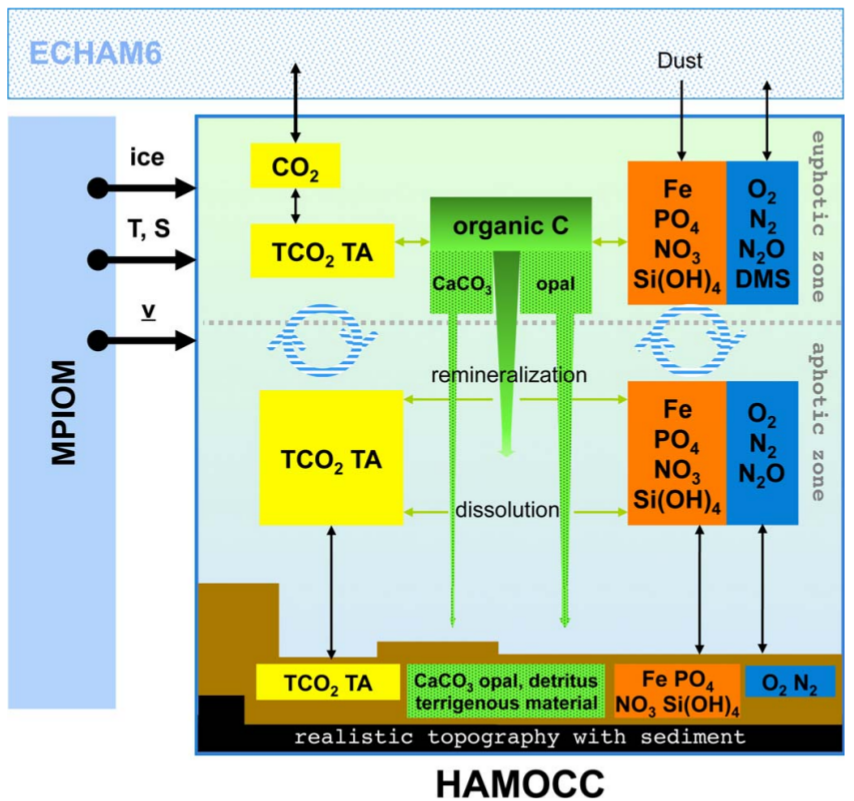
\includegraphics[scale=.4]{hamocc.png}
	\caption{A schematic overview of the global ocean biogeochemistry model HAMOCC \citep{Ilyina2013}}
	\label{fig:HAMOCC}
\end{figure}

\subparagraph{misc/low impact on variability: chemistry, sediment}
Other processes in a biogeochemical model act on longer timescales or small amplitude and hence lack a strong signal in the carbon cycle. 

The chemistry in HAMOCC is modeled in the carbonate system and keeps track of alkalinity. Dissolved inorganic carbon and pH (*check that*)are directly calculated and other information derived from that.

For falling detritus, there exist two different parts: opal producing if silicate is available or calcium carbonate producing. Calcification then changes the alkalinity and carbon budget.

Once detritus reach the the ocean floor, particulate matter enters the sediment and finally the burial layer. At the boundary of the sediment, all tracers are in exchange with the sediment which via pore water exchange \citep{Heinze1991}.





\subsection{Large ensemble}
\paragraph{general: what is it? how produced technically?}
Large ensemble simulation are a novel tool to investigate internal variability. By repeating a climate simulation with an identical forcing and model code but changing the initial conditions slightly, single ensemble members will be exposed to the same process implementations but the interplay are a stochastically random level lets each realisation evolve in a unique way while still being bound to a common forced trend.
 
The MPI-ESM Large Ensemble (MPI-ESM LE) contains 100 simulations under historical CMIP5 forcing from 1850 to 2005 and is extended under Representative Concentration Pathway (RCP) 4.5 scenario until 2100. Ensemble members differ through starting from different year of the pre-industrial control simulation, so ocean and atmosphere have different initial conditions in each run. This was achieved by branching off ensemble members from the control run after roughly 50 years by increasing the atmospheric pCO$_2$ levels.

MPI-ESM LE data already provided data to a few MPI-M publications, e.g. \citep{Marotzke2015,Bittner2016}.

\paragraph{novel method: how are other ensembles different?} 
As large ensemble research is a recent feature due to powerful upscaling of super-computing facilities, the number of ensemble datasets is limited and published papers infrequent.

NCAR's Community Earth System Model large ensemble (CESM LE) \citep{Kay2015} underlies the pioneering internal variability studies of \citeauthor{Deser2012}. The initial state of the atmosphere  was slightly pertubed by roundoff-level changes to air temperature in their 32 runs. CESM LE served for studies analyzing the timescales of dection of trend in the ocean carbon sink \citep{McKinley2016} and the partioning if its uncertainties \citep{Lovenduski2016}.

GFDL ran a 30-member ensemble simulation based on their model ESM2M. They use different dates separated by one day each but didn't publish any oceanic carbon uptake paper \citep{Rodgers2015}.

Previous studies assume gaussian statistics, but lack an adequate ensemble size to check for in detail \citep{Thompson2015,Deser2012} (see \ref{fig:SOCS_temporal_gaussian}).


\subsection{Data}
\paragraph{where are they from and why I choose this product?}
For comparison of CO$_2$flux with model simulations, I use the SOM-FFN data  which is based on the Surface Ocean Atlas Version 4 (SOCATv4) \citep{landschuetzer2016}. It uses a neural network-based data interpolation to create pCO$_2$ maps \citep{Landschuetzer2014}. The data product is smoothed by a 3x3 filter averaging two months and the neighboring grid cells, but this has little effect on seasonal dynamics. I use this pCO$_2$ data product because it seems a smart interpolation of pCO$_2$ data to cover regions without direct pCO$_2$ measurements. However, the input training data of the algorithm is seasonally biased, as the available pCO$_2$ samples originate mostly from austral summer months.



\clearpage

\section{Historical evolution of the Southern Ocean carbon sink}

\paragraph{carbon sink SO: forced trend and int variability, int var results} explain fig. \ref{fig:evolution_southern_ocean_carbon_sink}; 
Internal variability, defined as the 1$\sigma$-spread of the 100-members, is constant over this period (~0.18 $\pm$ 0.02 PgC yr$^{-1}$).
why can I do that:refer fig. \ref{fig:SOCS_temporal_gaussian} 

\paragraph{comparison ensemble to data} SOM-FFN data ranges within the 2$\sigma$ ensemble spread. We find carbon trends similar to those in the 1990s and 2000s. 


\paragraph{choice of trends: compromise signal strength and signal monotonic length; describe selection technical} compromise between decade=10yrs vs interannual variability, not too strong influence of atmospheric forced trend and strength of signal Fig \ref{fig:heatmap}; Exemplary for all decadal carbon sink trend ensemble members, I show the most extreme cases. The underlying mechanisms for carbon sink trends in our ensemble simulation seem to be of the same origin regardless of the exact trend period.


\begin{figure}[h!]
	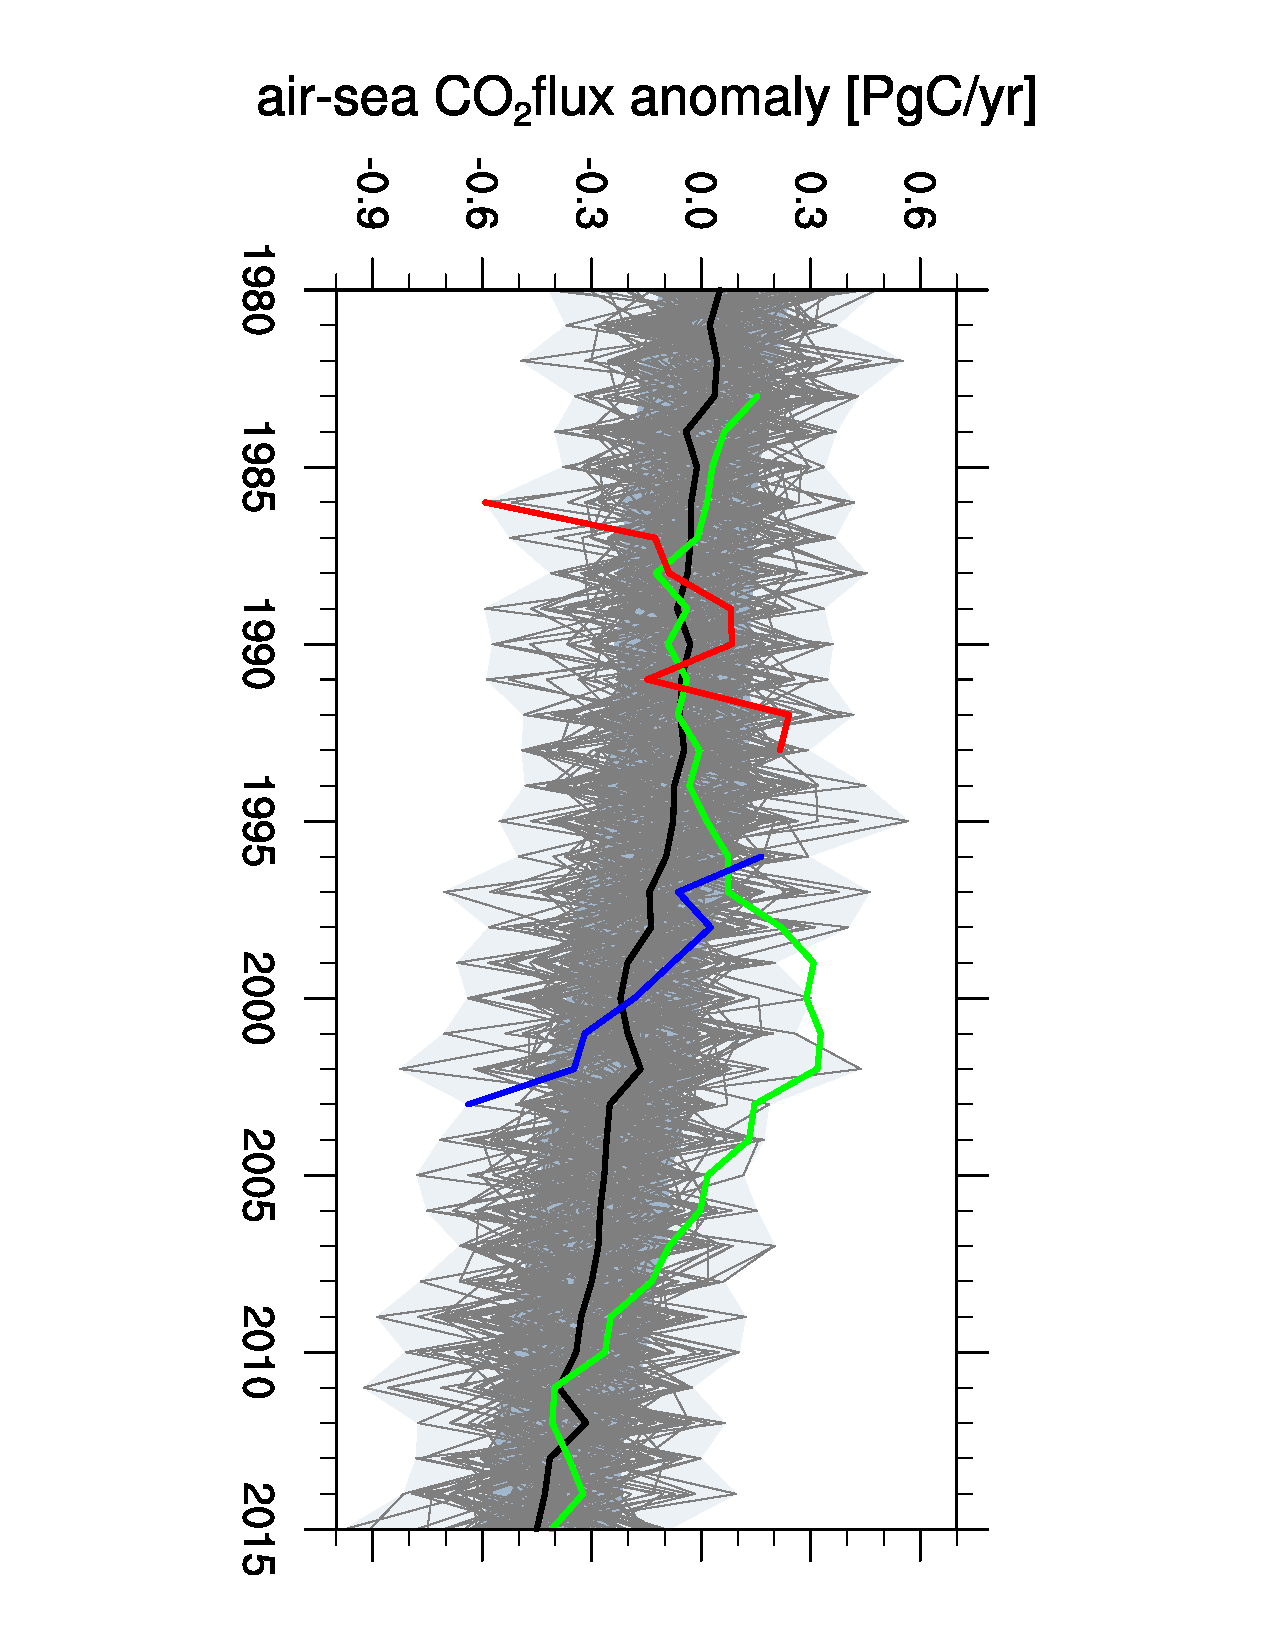
\includegraphics[scale=.55,angle=90,trim=4cm 0cm 4cm 0cm,clip]{co2flux_SO_timeseries_ymjm_35S_1980_2015_trend_8}
	\caption{Evolution of the Southern Ocean carbon sink anomaly south of 35$^\circ$S. Grey lines show the 100 ensemble members, the black line the ensemble median, the gray shading is the range of the ensemble, the blue shading is the 1$\sigma$ ensemble spread, the red line shows a positive sink trend, the blue line shows a negative sink trend, the green line represents the SOM-FFN observation-based estimate \citep{landschuetzer2015}; negative values indicate anomalous uptake with respect to the 1980s}
\label{fig:evolution_southern_ocean_carbon_sink}
\end{figure}


\paragraph{timeseries sam, biology, upwelling index? nice-to-have, but no connection to storyline; temporal results: seems short}


%\begin{figure}[h!]
%\includegraphics[scale=.55,angle=90,trim=4cm 0cm 4cm 0cm,clip,page=2]{co2flux_SO_timeseries_ymjm_35S_1980_2015_trend_8}
%\includegraphics[scale=.55,angle=90,trim=4cm 0cm 4cm 0cm,clip,page=3]{co2flux_SO_timeseries_ymjm_35S_1980_2015_trend_8}
%\caption{Evolution of the Southern Ocean primary production south of 35$^\circ$S and SAM. Grey lines show the 100 ensemble members, the black line the ensemble median, the gray shading is the range of the ensemble, the blue shading is the $\sigma$ ensemble spread, the red line reprensents negative carbon sink trend, the blue line represents positive carbon sink trend}
%\label{fig:evolution_southern_ocean_intpp}
%\end{figure}

\paragraph{transition to process understanding in spatial view; afterwards only two members shown exemplarily}
As shown in previous studies \citep{LeQuere2007}, the variations of oceanic carbon uptake are related to the background thermal and dynamic changes. Some note on biology refering to hypothesis?


\clearpage

\section{Spatial distribution of Southern Ocean carbon sink}


\paragraph{mean state and internal variability Southern ocean carbon sink} 
refer to fig. \ref{fig:SOCS_ensmean_ensstd}

\paragraph{mean state and internal variability Southern ocean westerly winds? no plot yet}

\paragraph{mean state and internal variability of biology and link to carbon sink} 
refer to fig. \ref{fig:SOCS_ensmean_ensstd}

\paragraph{mean state and internal variability of upper ocean circulation and link to carbon sink}
refer to fig. \ref{fig:UOOC_mean}


\begin{figure}[h!]
\centering
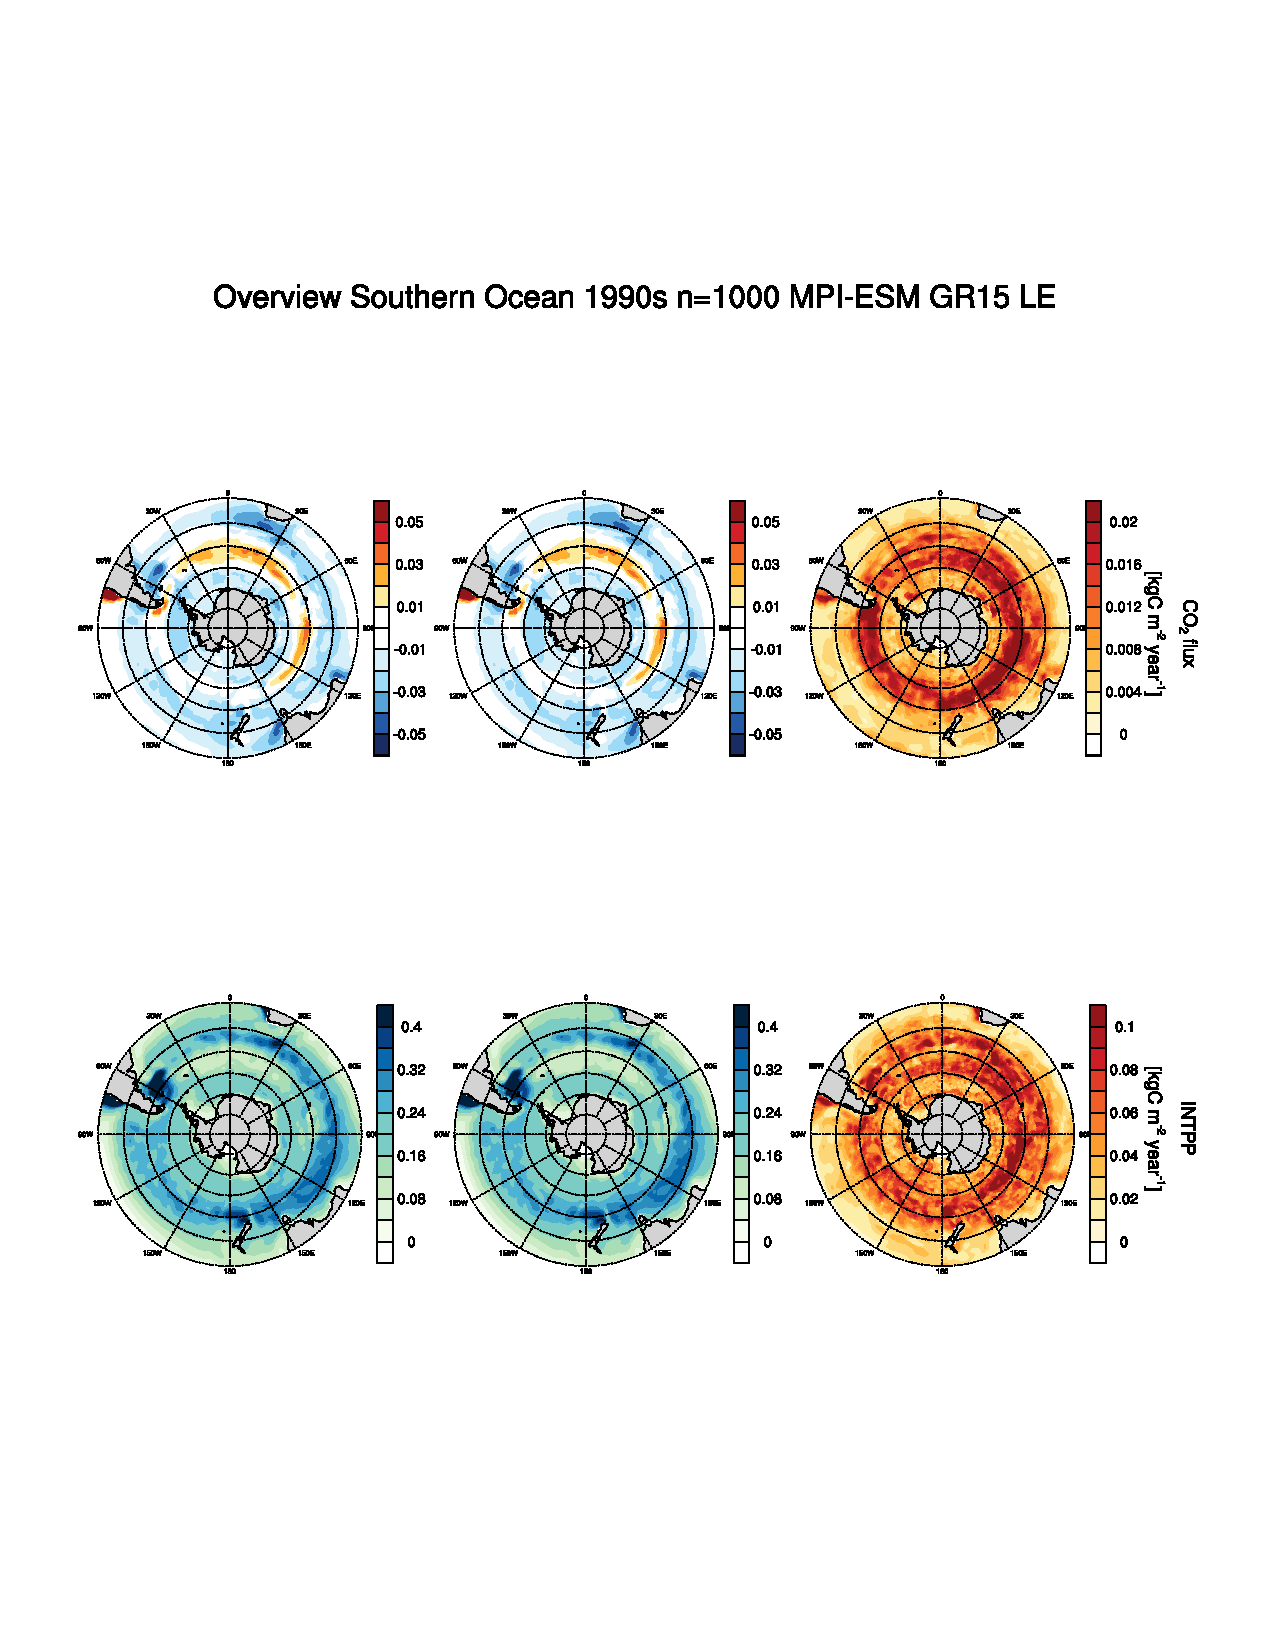
\includegraphics[scale=1.,trim=7.2cm 15cm 0cm 8cm,clip]{Overview_SO_co2flux_intpp_ens_t1990s.pdf} % co2flux
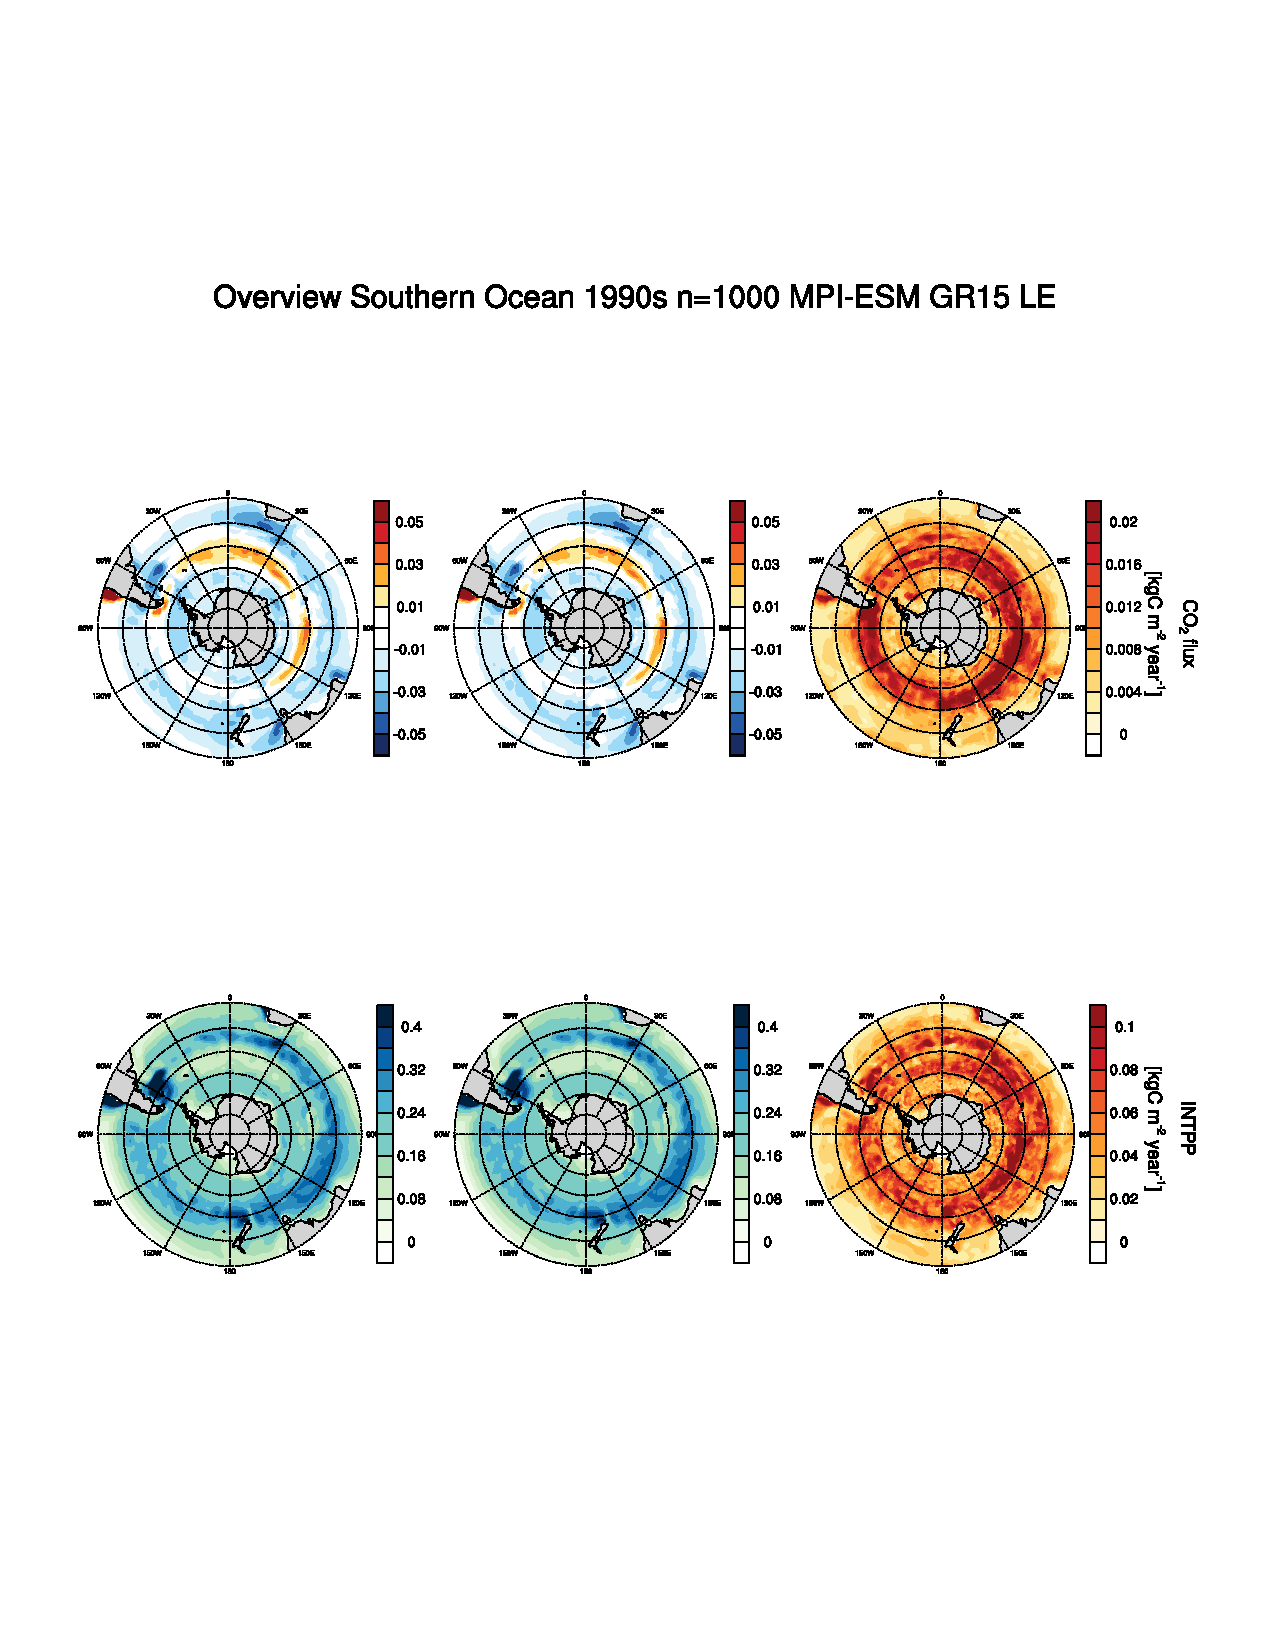
\includegraphics[scale=1.,trim=7.2cm 6.3cm 0cm 16cm,clip]{Overview_SO_co2flux_intpp_ens_t1990s.pdf} % intpp
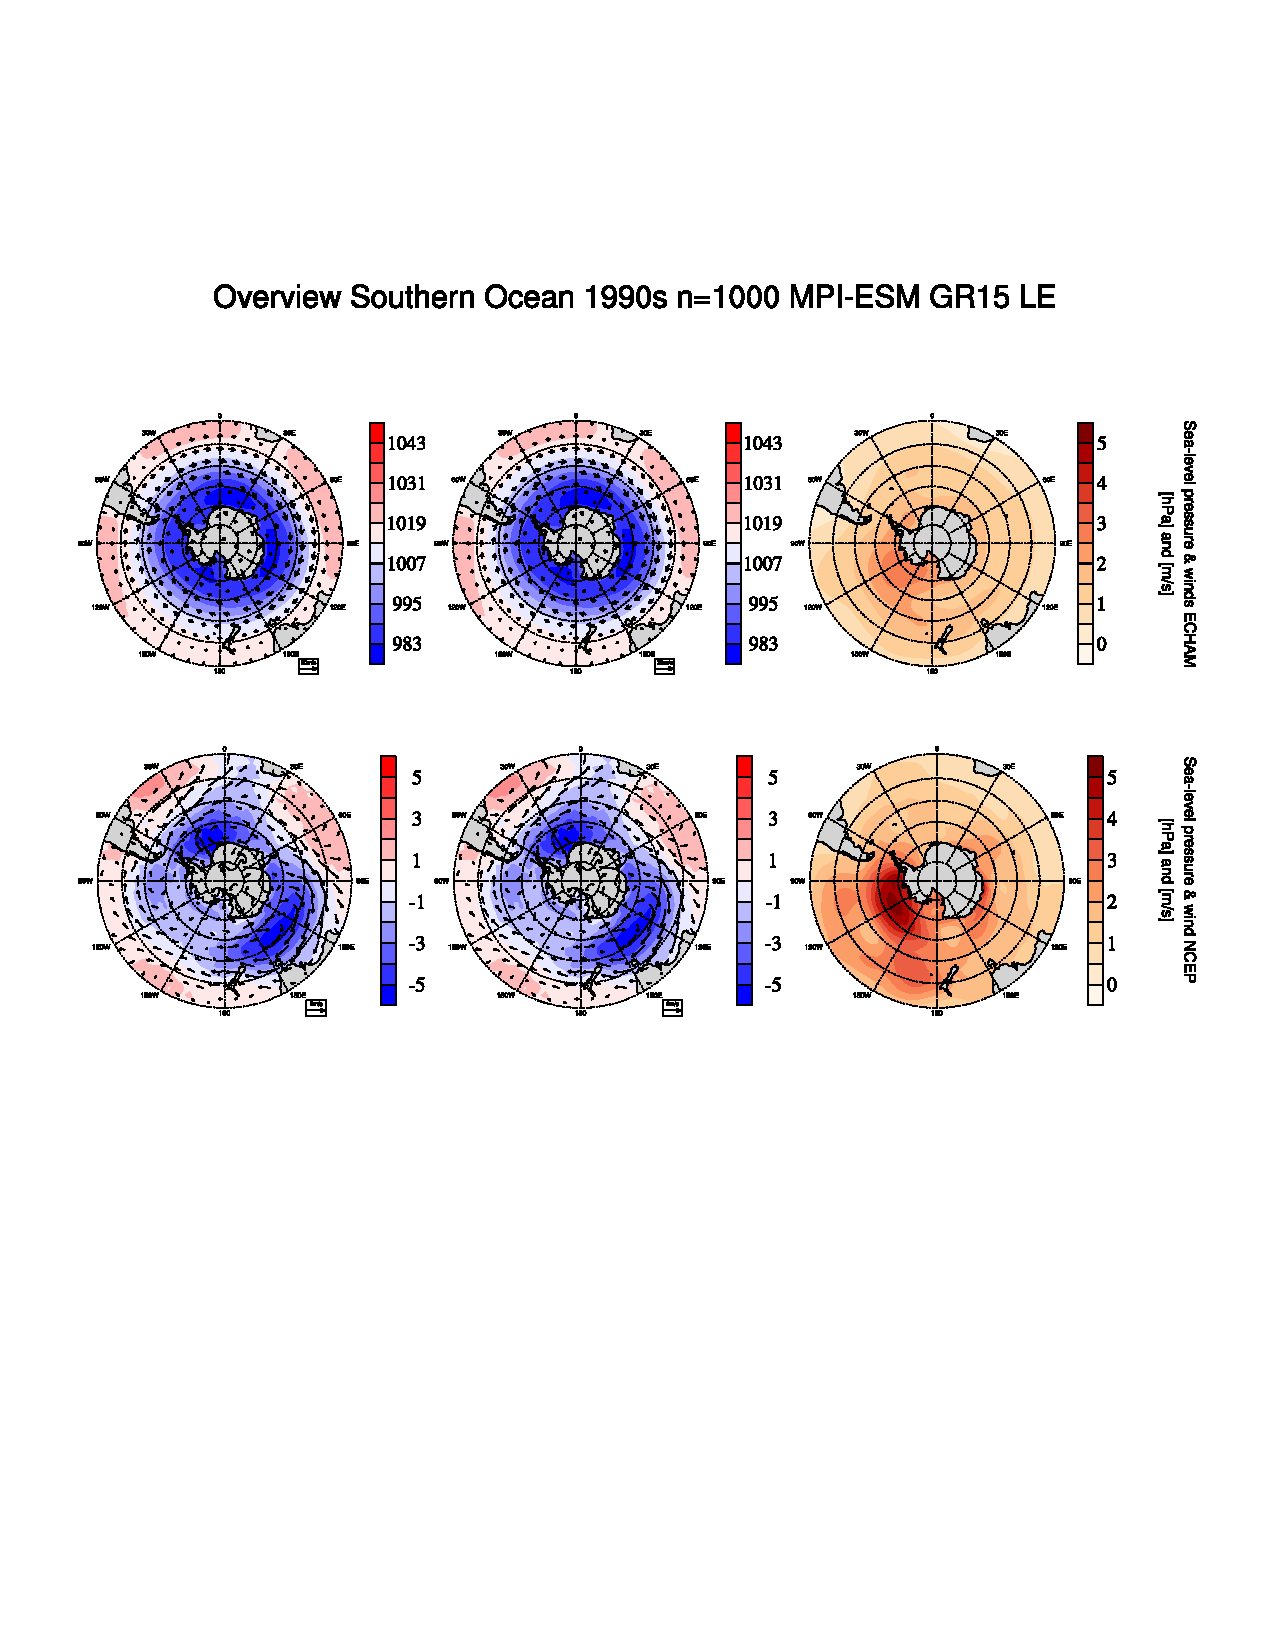
\includegraphics[scale=1.,trim=7.2cm 15cm 0cm 8cm,clip]{Overview_SO_slp_ens_t1990s.pdf} % slp
\caption{Spatial distribution of the yearmean Southern Ocean CO$_2$flux (top) and primary production (bottom): negative values indicate ocean uptake ensemble median (left) as forced signal and ensemble standard deviation (right) as internal variability}
\label{fig:SOCS_ensmean_ensstd}
\end{figure}



\begin{figure}[h!]
\centering
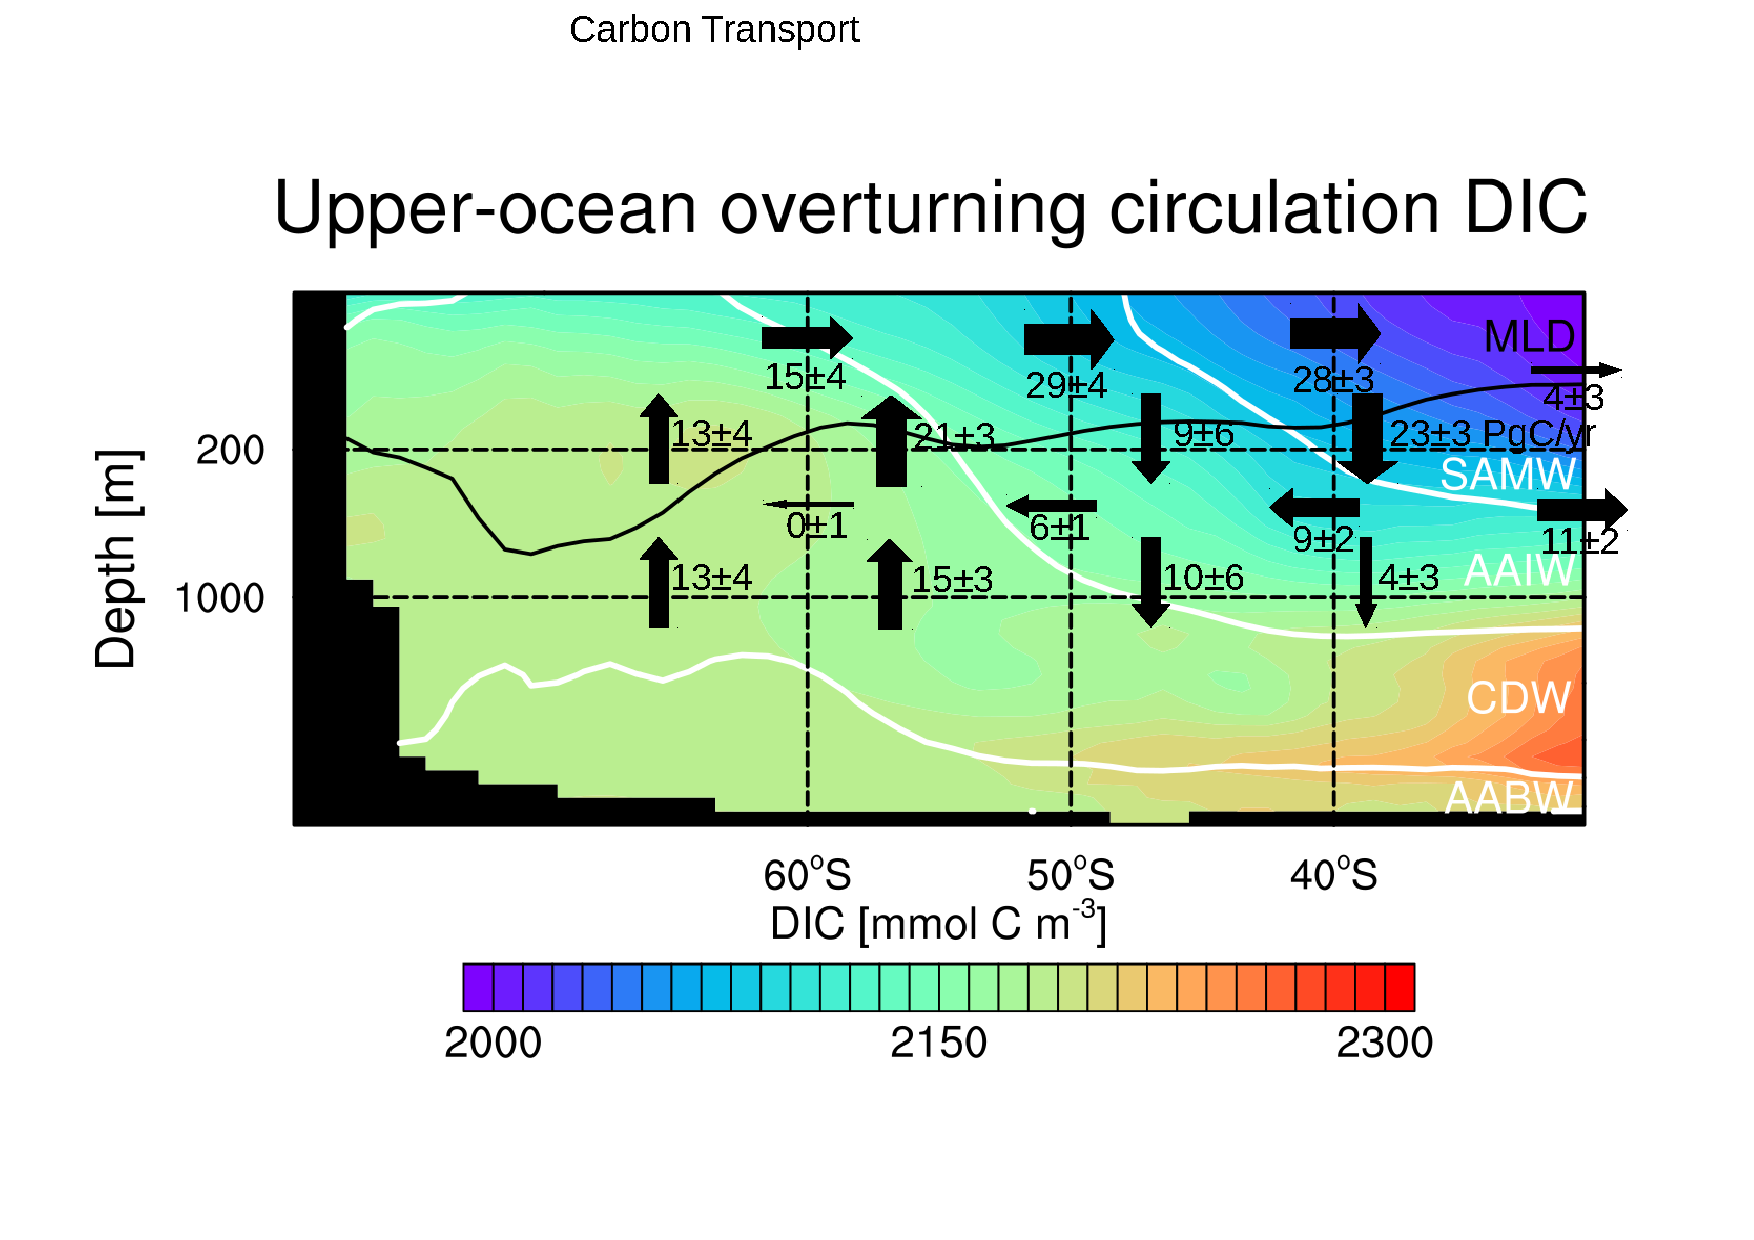
\includegraphics[scale=0.5,page=1,trim=1.4cm 1.7cm 0cm 4.6cm,clip]{UOOC}
\vspace{-8mm}
\caption{Upper-ocean overturning circulation modulates the carbon sink as carbon-rich water are upwelled and carbon-depleted water are downwelled; black arrows show yearly mean advective carbon transport; white lines are isopyncals separating Sub-Antarctic Mode Water (SAMW), Antarctic Intermediate Water (AAIW), Circumpolar Deep Water (CDW) and Antarctic Bottom Water (AABW)}
	\label{fig:UOOC_mean}
\end{figure}










\clearpage

\subsection{Negative trends in carbon sink}


\paragraph{trends in pCO2 and westerly winds} refer fig. \ref{fig:pco2_neg} 

pCO2 (and not co2flux) to show co2flux not only increasing due to stronger winds only by formula
 The region of 50-60$^\circ$S has the strongest decreasing trend in CO$_2$flux. leads to hypothesis
 
\paragraph{schematics: explain carbon decrease due to wind} refer to fig. \ref{fig:schematics_stronger_winds} - can I show this already here or better after the plots 



\begin{figure}[h!]
\centering
	\includegraphics[scale=.8,trim=8cm 14.5cm 8cm 6.4cm,clip]{\memberpositive _positive_trend_8_Landschuetzer_overview.pdf}
	\includegraphics[scale=1.,trim=8cm 4.5cm 8cm 17.9cm,clip]{\memberpositive _positive_trend_8_Landschuetzer_overview.pdf}	
	\caption{pCO$_2$(right) (left) and Trends in sea-level pressure and winds - should I also discuss thermal and non-thermal trends in \citep{landschuetzer2015}?}
	\label{fig:pco2_neg}
\end{figure}




\begin{figure}[h!]
	\centering
	\includegraphics[scale=.4,trim=2cm 3.5cm 2cm 2cm,clip,page=5]{SO_schematics}
	\caption{Schematic illustration of the Southern Ocean under the context of increasing westerly winds and response of biology and upper-ocean circulation towards the carbon sink}
	\label{fig:schematics_stronger_winds}
\end{figure}


\subsubsection{Changes in biology in negative CO$_2$flux trends}

\paragraph{on trends in co2flux, intpp} Primary production and CO$_2$flux show opposing trend patterns as plankton growth takes up large amounts of surface DIC and hence lowers pCO$_2$

\paragraph{on intpp not increasing because of more nutrients} different than \citep{Lovenduski2005} (can I cite this here or only in discussion? or rather cite paper about SO iron lack and increased iron supply from upwelling?)

\paragraph{on temp and light limitation changes due to SAM, coastal due to ice}

\paragraph{then why intpp decreases in 50s? zmld mixing and light depth limitation} Sverdrup \citep{Sverdrup1953} introduced his concept of critical depth based turbulent mixing as a requirement for plankton blooms \citep{Franks2014}

\begin{figure}[h!]
	\includegraphics[scale=1.4,trim=13.25cm 18.7cm 2.5cm 6cm,clip]{\memberpositive _positive_trend_8_obgc_overview_summer.pdf} %co2flux
	\includegraphics[scale=1.4,trim=13.25cm 15.9cm 2.5cm 9.2cm,clip]{\memberpositive _positive_trend_8_obgc_overview_summer.pdf} %intpp
	\includegraphics[scale=1.4,trim=13.25cm 13.1cm 2.5cm 12.1cm,clip]{\memberpositive _positive_trend_8_obgc_overview_summer.pdf} %nutlimf
	\includegraphics[scale=1.4,trim=13.25cm 7.3cm 2.5cm 17.8cm,clip]{\memberpositive _positive_trend_8_obgc_overview_summer.pdf} %zmld
	\includegraphics[scale=1.4,trim=13.25cm 10.15cm 2.5cm 14.9cm,clip]{\memberpositive _positive_trend_8_obgc_overview_summer.pdf} %temp
	\includegraphics[scale=1.4,trim=13.25cm 4.5cm 2.5cm 20.65cm,clip]{\memberpositive _positive_trend_8_obgc_overview_summer.pdf} %light
	\includegraphics[scale=.5,trim=1.2cm 13.2cm 11cm 7cm,clip]{\memberpositive _positive_trend_8_schwerpunkt_mixing_overview.pdf} % intpp depth
	\hspace{3.5cm}
	\includegraphics[scale=.5,trim=11cm 13.2cm 0cm 7cm,clip]{\memberpositive _positive_trend_8_schwerpunkt_mixing_overview.pdf} % wind penetration depth
	\caption{Southern Ocean austral summer trends per 8 years: CO$_2$flux (top left), vertically integrated primary production (top right), nutrient limitation (middle right), mixed layer depth (middle left), temperature limitation function (bottom left) and light limitation function (bottom right); Trends in [m/8yrs] for phytoplankton average depth (left) and average depth of vertical diffusivity due to wind (right); hatched areas indicate where trends were below 5\% significance}
	\label{fig:co2flux_intpp_neg}
\end{figure}


\paragraph{center of mass of phytoplankton and wind penetration depth}
refer fig. \ref{fig:co2flux_intpp_neg} 

%\begin{figure}[h!]
%	\centering
%	\includegraphics[scale=.5,trim=1.2cm 13.2cm 0cm 7cm,clip]{\memberpositive _positive_trend_8_schwerpunkt_mixing_overview.pdf}
%	\caption{Trends in [m/8yrs] for phytoplankton average depth (left) and average depth of vertical diffusivity due to wind (right); hatched areas indicate where trends were below 5\% significance}
%	\label{fig:wind_mixing_neg}
%\end{figure}


\paragraph{concentration increase of intpp at 40s due to advection/ekman transport} refer fig. \ref{fig:ekman_neg}



\clearpage



\subsubsection{Changes in ocean circulation in negative CO$_2$flux trends}

\paragraph{transition: zmld trends; Upper-ocean overturning circulation: up, ekman transport, downwelling} The strong trend in MLD could also be a sign of increasing outgassing due to more mixing (fig. \ref{fig:co2flux_intpp_neg}). refer to fig. \ref{fig:ekman_neg}
temperature pump effect?

\begin{figure}[h!]
	\centering
	\includegraphics[scale=1.2,trim=13.25cm 18.7cm 3.5cm 6cm,clip]{\memberpositive _positive_trend_8_ekman_overview.pdf}
	\includegraphics[scale=1.2,trim=13.25cm 15.9cm 3.5cm 9.2cm,clip]{\memberpositive _positive_trend_8_ekman_overview.pdf}
	\caption{Ekman transport and ekman upwelling trends}
	\label{fig:ekman_neg}
\end{figure}


\paragraph{carbon transport changes}
refer fig. \ref{fig:UOOC_neg}

\begin{figure}[h!]
	\centering
	\includegraphics[scale=0.4,page=2,trim=1.4cm 1.7cm 0cm 4.6cm,clip]{UOOC}
	\vspace{-5mm}
	\caption{Increased upper-ocean overturning circulation weakens the carbon sink as carbon-rich water are upwelled and carbon-depleted water are downwelled}%; black arrows show mean advective carbon transport, red arrows show advective carbon transport trend over 8 years; white lines are isopyncals separating Sub-Antarctic Mode Water (SAMW), Antarctic Intermediate Water (AAIW), Circumpolar Deep Water (CDW) and Antarctic Bottom Water (AABW)}
	\label{fig:UOOC_neg}
\end{figure}













\clearpage

\subsection{Positive trends in carbon sink}

\paragraph{disclaimer: everything upside down}

\paragraph{trends in pCO2 and westerly winds} refer fig. \ref{fig:pCO2_pos} 
 The region of 50-60$^\circ$S has the strongest decreasing trend in CO$_2$flux. leads to hypothesis
 
\paragraph{schematic changes due to wind} refer to fig. \ref{fig:schematics_weaker_winds} 


\begin{figure}[h!]
	\centering
	\includegraphics[scale=.8,trim=8cm 14.5cm 8cm 6.4cm,clip]{\membernegative _positive_trend_8_Landschuetzer_overview.pdf}
	\includegraphics[scale=1.1,trim=8cm 4.5cm 8cm 17.9cm,clip]{\membernegative _positive_trend_8_Landschuetzer_overview.pdf}
	\caption{Trends in pCO$_2$ (left) and sea-level pressure and winds (right)}
	\label{fig:pCO2_pos}
\end{figure}


\begin{figure}[h!]
	\centering
\includegraphics[scale=.45,trim=2cm 3.5cm 2cm 2cm,clip,page=9]{SO_schematics}
	\caption{Schematic illustration of the Southern Ocean under the context of decreasing westerly winds}
	\label{fig:schematics_weaker_winds}
\end{figure}



\clearpage

\subsubsection{Changes in biology in positive CO$_2$flux trends}

\paragraph{on trends in co2flux, intpp} Primary production and CO$_2$flux show opposing trend patterns as plankton growth takes up less surface DIC and hence pCO$_2$ increases fig. \ref{fig:pCO2_pos}. refer to fig. \ref{fig:co2flux_intpp_pos} 


\paragraph{on intpp not decreasing because of less nutrients}  different than \citep{Lovenduski2005} (can I cite this here or only in discussion?)

\paragraph{on temp and light limitation changes due to SAM, coastal due to ice}

\paragraph{the why intpp increases in 50s: using less zmld mixing} refer fig. \ref{fig:co2flux_intpp_pos}

\begin{figure}[h!]
	\includegraphics[scale=1.4,trim=13.25cm 18.7cm 2.5cm 6cm,clip]{\membernegative _positive_trend_8_obgc_overview_summer.pdf} %co2flux
	\includegraphics[scale=1.4,trim=13.25cm 15.9cm 2.5cm 9.2cm,clip]{\membernegative _positive_trend_8_obgc_overview_summer.pdf} %intpp
	\includegraphics[scale=1.4,trim=13.25cm 13.1cm 2.5cm 12.1cm,clip]{\membernegative _positive_trend_8_obgc_overview_summer.pdf} %nutlimf
	\includegraphics[scale=1.4,trim=13.25cm 7.3cm 2.5cm 17.8cm,clip]{\membernegative _positive_trend_8_obgc_overview_summer.pdf} %zmld
	\includegraphics[scale=1.4,trim=13.25cm 10.15cm 2.5cm 14.9cm,clip]{\membernegative _positive_trend_8_obgc_overview_summer.pdf} %temp
	\includegraphics[scale=1.4,trim=13.25cm 4.5cm 2.5cm 20.65cm,clip]{\membernegative _positive_trend_8_obgc_overview_summer.pdf} %light
	\includegraphics[scale=.5,trim=1.2cm 13.2cm 11cm 7cm,clip]{\membernegative _positive_trend_8_schwerpunkt_mixing_overview.pdf} % phy depth
	\hspace{3.5cm}
	\includegraphics[scale=.5,trim=11cm 13.2cm 0cm 7cm,clip]{\membernegative _positive_trend_8_schwerpunkt_mixing_overview.pdf} % wind penetration depth
	\caption{Southern Ocean austral summer trends per 8 years: CO$_2$flux (top left), vertically integrated primary production (top right), nutrient limitation (middle right), mixed layer depth (middle left), temperature limitation function (bottom left) and light limitation function (bottom right); Trends in [m/8yrs] for phytoplankton average depth (left) and average depth of vertical diffusivity due to wind (right); hatched areas indicate where trends were below 5\% significance}
\label{fig:co2flux_intpp_pos}
\end{figure}

%\begin{figure}[h!]
%	\centering
%	\includegraphics[scale=.5,trim=1.2cm 13.2cm 0cm 7cm,clip]{\membernegative _positive_trend_8_schwerpunkt_mixing_overview.pdf}
%%	\includegraphics[page=2,scale=.25,trim=0cm 6cm 0cm 5cm,clip]{\membernegative _positive_trend_8_seasonality_intpp_zmld.pdf} % from gfx folder
%	\caption{Trends in [m/8yrs] for phytoplankton average depth (left) and average depth of vertical diffusivity due to wind (right); hatched areas indicate where trends were below 5\% significance}
%	\label{fig:wind_mixing_pos}
%\end{figure}




\clearpage

\subsubsection{Changes in ocean circulation in positive CO$_2$flux trends}

\paragraph{transition: zmld trends; Upper-ocean overturning circulation: up, ekman transport, downwelling} 
The strong  stabilizing trend in MLD could also be a sign of decreasing outgassing due to less mixing (fig. \ref{fig:co2flux_intpp_pos}). refer to fig. \ref{fig:ekman_pos} temperature pump effect?

\begin{figure}[h!]
	\centering
	\includegraphics[scale=1.6,trim=13.25cm 18.7cm 3.5cm 6cm,clip]{\membernegative _positive_trend_8_ekman_overview.pdf}
	\includegraphics[scale=1.6,trim=13.25cm 15.9cm 3.5cm 9.2cm,clip]{\membernegative _positive_trend_8_ekman_overview.pdf}
	\caption{Ekman transport and ekman upwelling trends}
	\label{fig:ekman_pos}
\end{figure}


\paragraph{carbon transport changes}
refer fig. \ref{fig:UOOC_pos}


\begin{figure}[h!]
	\centering
	\includegraphics[scale=0.5,page=3,trim=1.4cm 1.7cm 0cm 4.6cm,clip]{UOOC}
	\vspace{-5mm}
	\caption{Decreased upper-ocean overturning circulation strengthens the carbon sink as carbon-rich water are less upwelled and carbon-depleted water are less downwelled - background is static and not this specific member, ok?}%; black arrows show mean advective carbon transport, red arrows show advective carbon transport trend over 8 years; white lines are isopyncals separating Sub-Antarctic Mode Water (SAMW), Antarctic Intermediate Water (AAIW), Circumpolar Deep Water (CDW) and Antarctic Bottom Water (AABW)}
	\label{fig:UOOC_pos}
\end{figure}




\clearpage

\section{50-60S dominates Internal Variability of the total Southern Ocean carbon sink due to winds - need a better title: emphasis on 50S as driving int var region via winds}

\paragraph{on area 50-60S as driver of Southern Ocean internal variability, correlation plots co2flux and wind trends} fig. \ref{fig:scatter} refer to fig. \ref{fig:schematics_stronger_winds} and fig. \ref{fig:schematics_weaker_winds}
stronger winds isopycnal movement \citep{Lauderdale2013}
\\ co2flux trend = (0.081$\pm$0.001) SAM trend 

\begin{figure}[h!]
\centering
		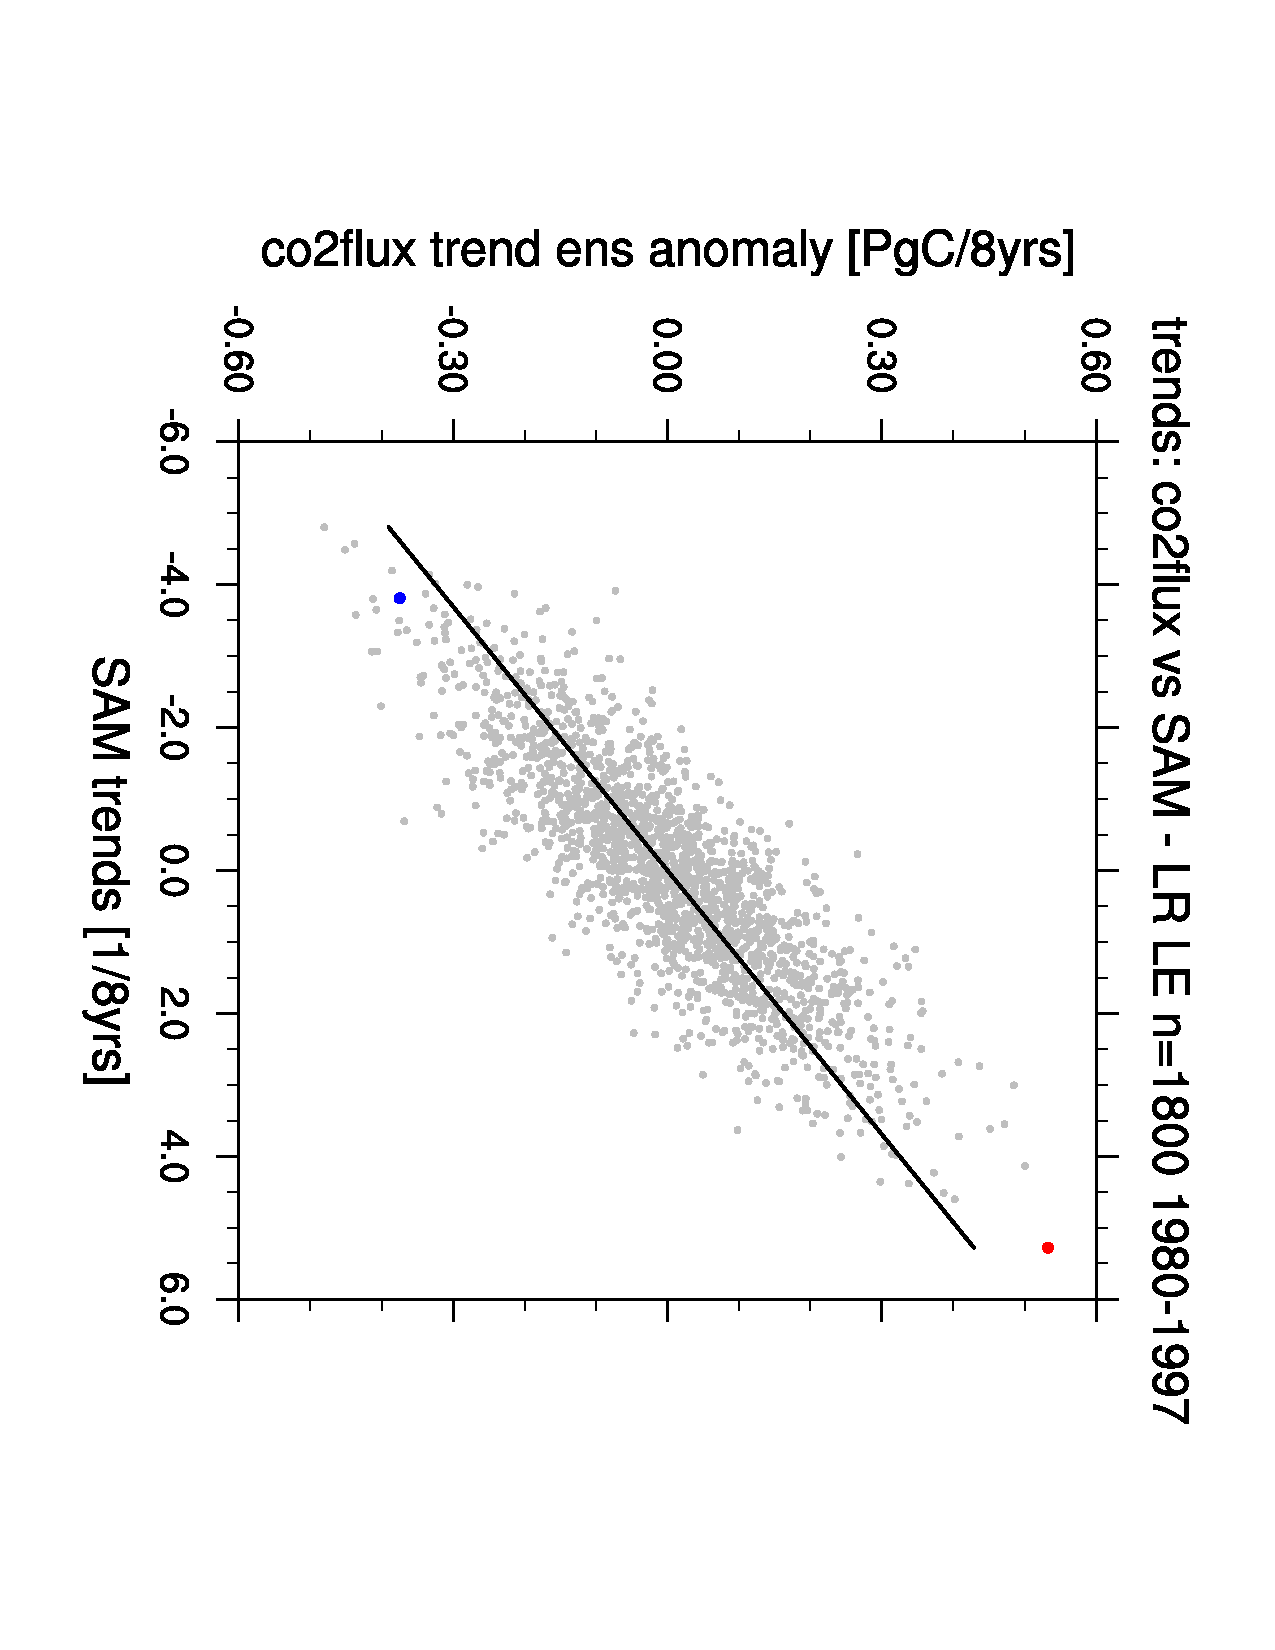
\includegraphics[scale=.7,page=1,angle=90,trim=1.3cm 2.3cm 2.3cm 3cm,clip]{Scatter_trends_bands_ensanom_co2flux_vs_SAM_n1800_1980_1997_trend8_50-59S}
		%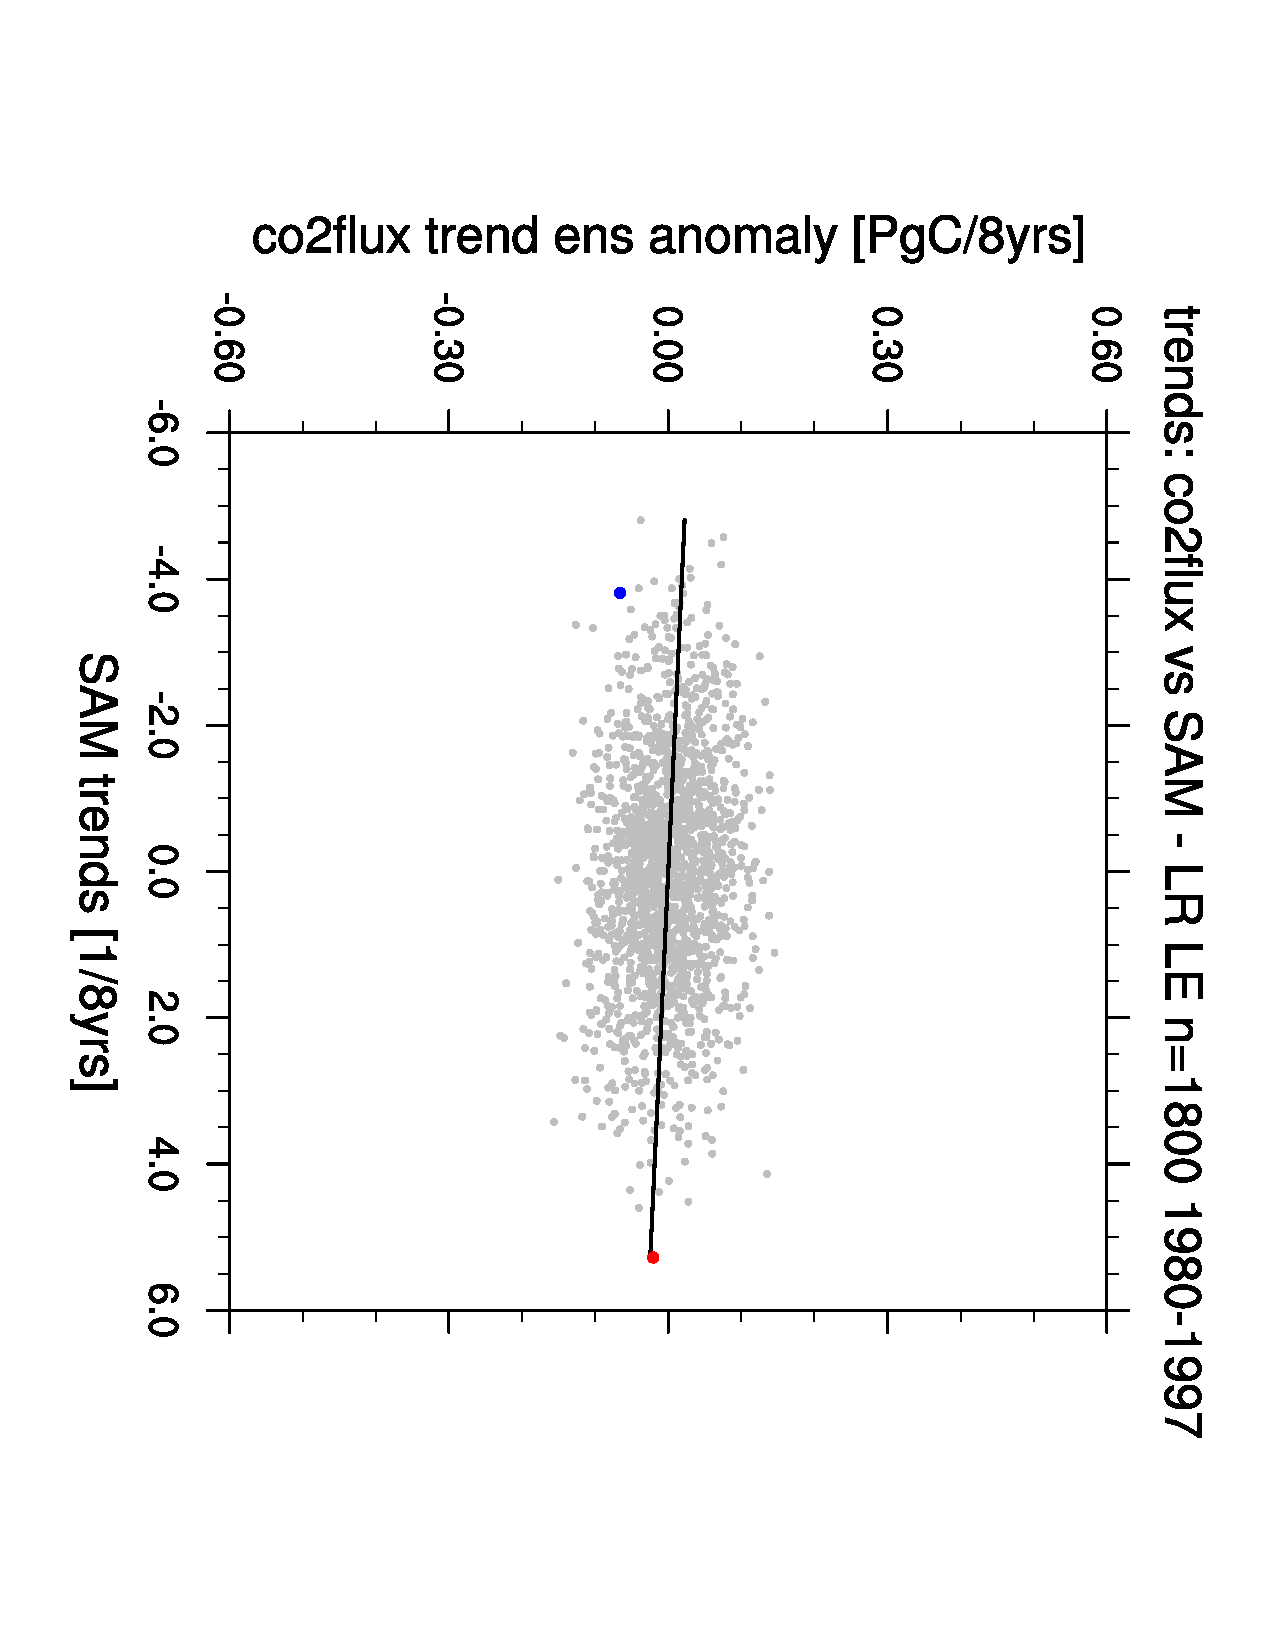
\includegraphics[scale=.38,page=1,angle=90,trim=1.3cm 2.3cm 2.3cm 3cm,clip]{Scatter_trends_bands_ensanom_co2flux_vs_SAM_n1800_1980_1997_trend8_40-49S}
		\vspace{-2mm}
		\caption{Southern Annular Mode (SAM) as indicator of wind strength vs. CO$_2$flux south of 35$^\circ$S; left 50-60s; right 40-50; one data point represents 8-year trends of single realization minus ensemble mean in 8-year periods between 1980 and 2005; green dot is negative trend example, red dot is positive trend example}
		\label{fig:scatter}
\end{figure}

\clearpage
\section{estimate: bio vs upwelling}
still have to come up with something like co2flux separation in \citep{Lauderdale2016a}; nice to have

\clearpage

\section{Discussion}

My results in perspective...
\subsection*{Here I compare to other paper's messages (and results), in Results I only cite papers to emphasize processes}

\paragraph{on comparison biology paper} Iron-hypothesis \citep{Martin1990} doesnt apply to HAMOCC; similar zmld co2flux response though location differs \citep{Lovenduski2005,Hauck2013,wang2012} 

\paragraph{on comparison circulation paper} upwelling found to be major carbon sink driver \citep{landschuetzer2015,LeQuere2007,Lovenduski2007}, upwelling location boundaries differ slightly, upwelling trends deeper into ocean \citep{DeVries2017} \\
idealised sensitivity studies of carbon due to wind changes \citep{Lauderdale2013}

\paragraph{on comparison earlier co2flux paper} trend in same order of magnitude reproduced; different 1980s anomaly \citep{LeQuere2007,Lovenduski2007,landschuetzer2015} also reference to Sarmiento ARGO estimates: strength: insitu two years; weakness: few floats for large areas; SOM-FFN 2016 might be seasonally biased; interactive carbon cycle produces 25\% higher internal variability \citep{Ilyina2013}  

\paragraph{on internal variability comparison} US models have tropical and indian pacific as dominating variability mode region, MPI has Southern Ocean, MPI has higher int var than CESM, but lower than GFDL \citep{Resplandy2015}

\paragraph{on ensemble comparisons} CESM LE cannot reproduce decadal trends [private communication] weak SO carbon sink \citep{McKinley2016} \\ no knowledge about GFDL \citep{Rodgers2015} 

\paragraph{on MPI-OM Southern Ocean performance evaluation papers}  \citep{Jungclaus2013,Sallee2013,Sallee2013a,Heuze2013,Stoessel2015} 

\paragraph{on HAMOCC SO performance} pCO2 comparison Takahashi or surface DIC GLODAP \citep{Ilyina2013} %or new comparison with Landschuetzer? 
%\\ nutrient (nitrate, phosphate vs silicate) distributions vs obs
\\ amplified seasonal cycle \citep{Nevison2016}, early HAMOCC tuned for NH \citep{Six1996} %; co2flux formula from 1992 standard use but updated \citep{Wanninkhof2013}




\clearpage

\section{Summary and conclusions}


\paragraph{what I did and internal variability value $\pm$} make sure three questions are answered

\paragraph{two wind regimes of internal variability} processes processes at 50-60S linking to wind and summarising results of figure \ref{fig:scatter}

\paragraph{outlook: large ensemble variability modeling}
Outlook paragraph on internal variability from large ensemble simulations; ICLE comparison Rodgers

\paragraph{outlook: observational focus on Southern Ocean} ARGO data and SOM-FFN combined longer timeseries


\clearpage

\baselineskip18pt
%\addbibresource{../Paper/SouthernOceanCarbonSink_new}
\bibliography{../Paper/SouthernOceanCarbonSink_new}

\bibliographystyle{abbrvnat}%unsrtnat}%abbrvnat}%plainnat}

\clearpage

\listoffigures

\clearpage

\section*{Supplementary information}

\subsection*{Statistics of Southern Ocean carbon sink}

\begin{figure}[h]
	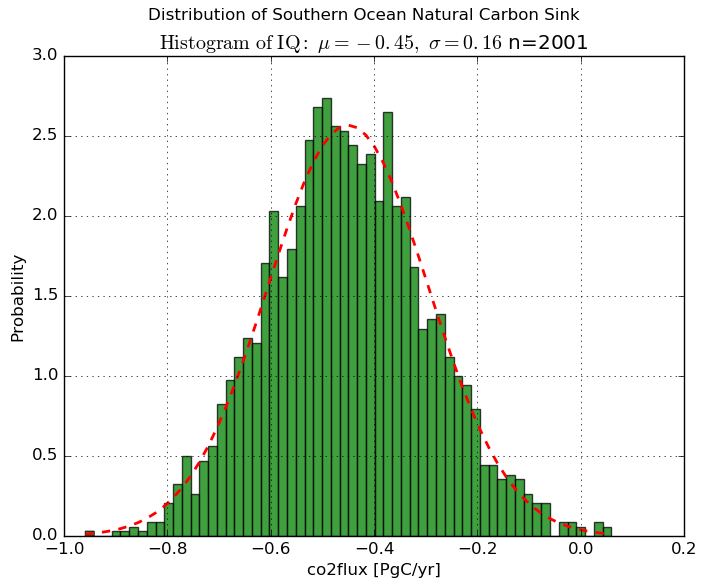
\includegraphics[scale=.4]{SOCS_temporal_gaussian.png} % from gfx folder
	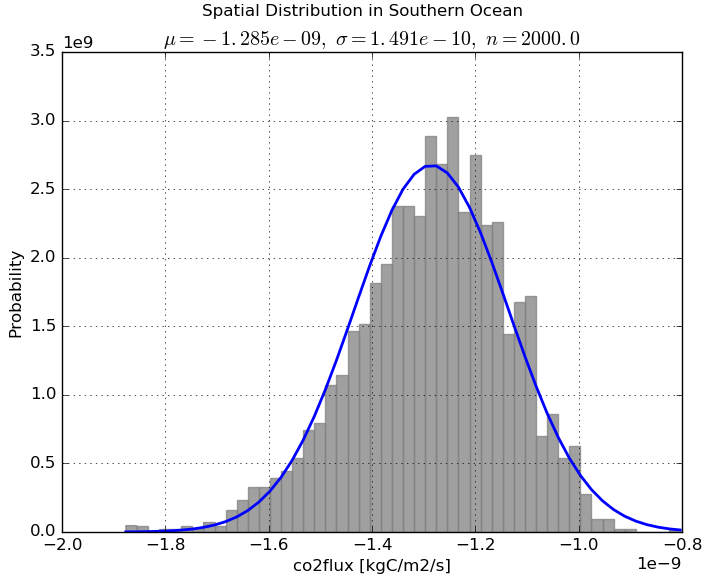
\includegraphics[scale=.4]{SOCS_spatial_gaussian.png} % from gfx folder
	\caption{Southern Ocean carbon sink: yearmean fieldsum 35-90S (left) and yearmean in a random grid cell (right)}
	\label{fig:SOCS_temporal_gaussian}
\end{figure}

\begin{figure}[h]
	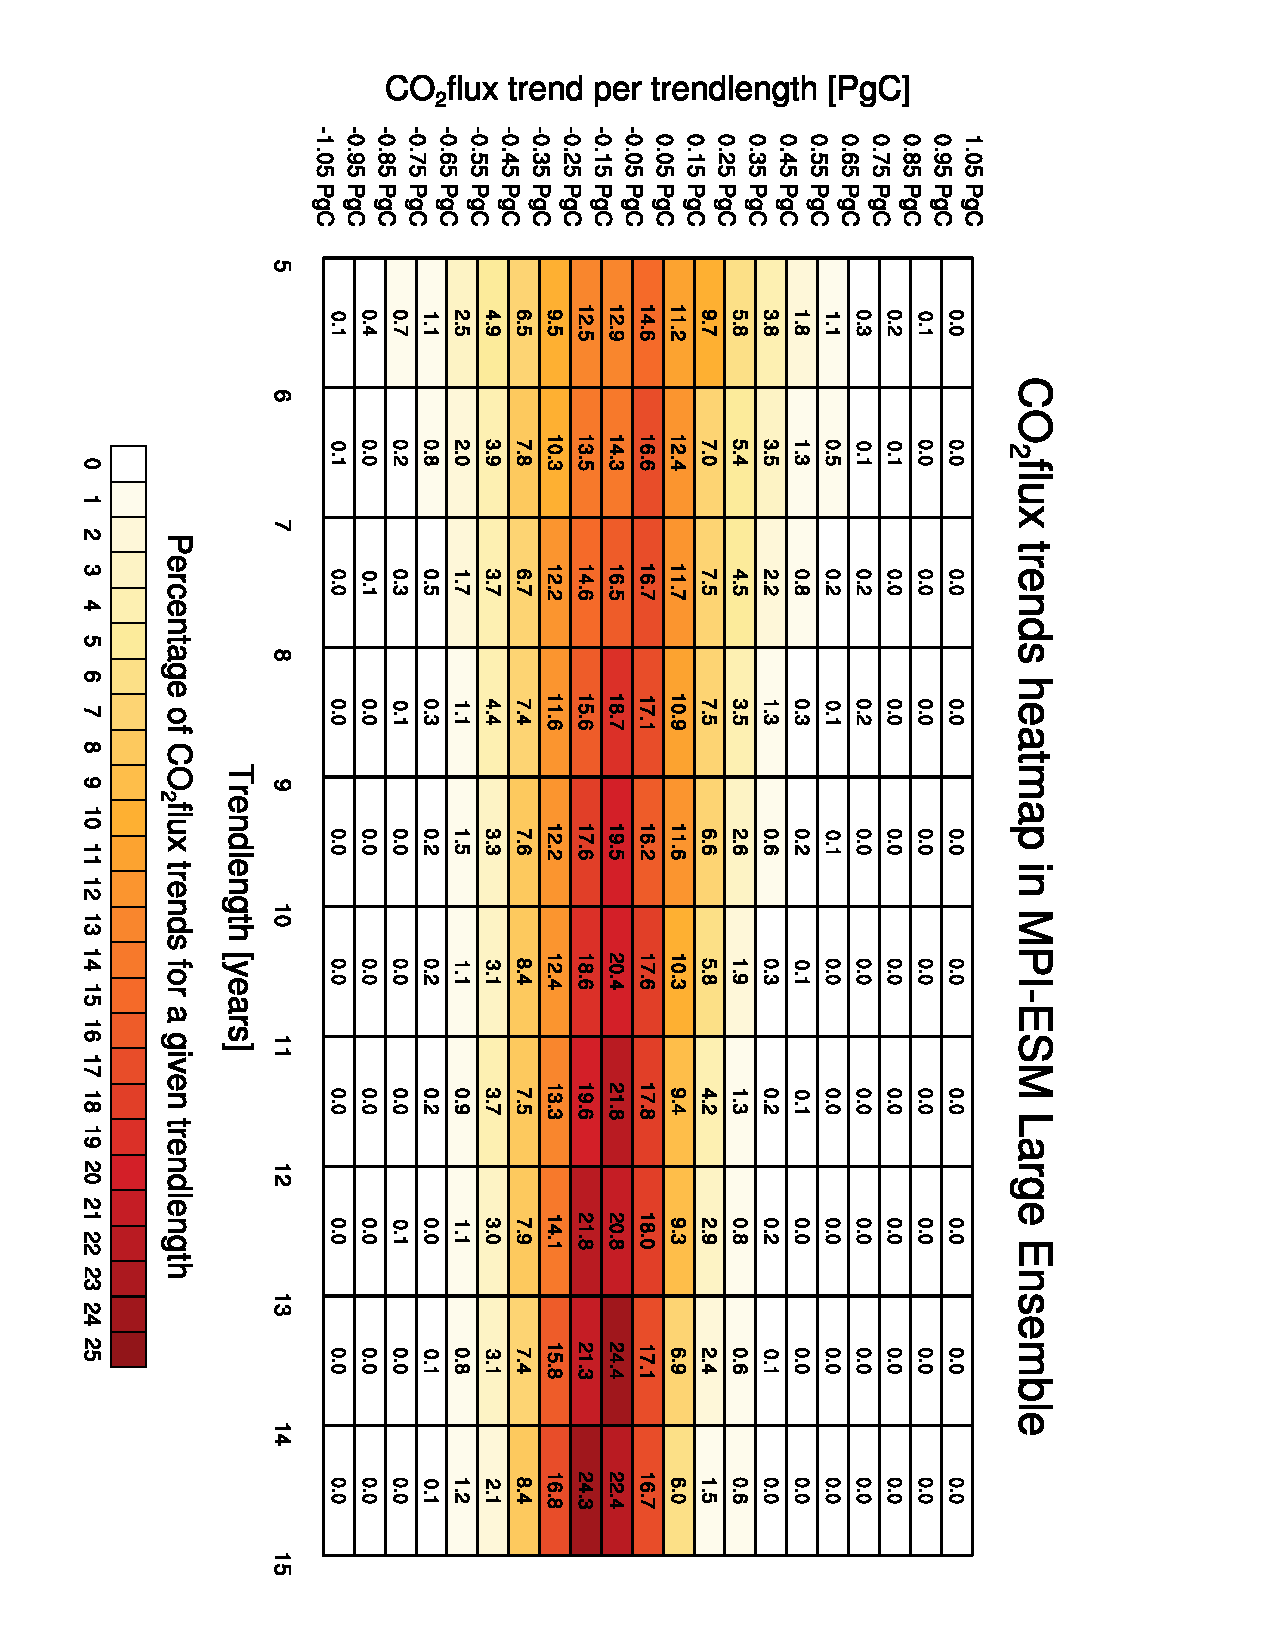
\includegraphics[scale=.64,angle=90,trim=5.3cm 1.3cm 1cm 1cm,clip]{heatmap_not_de-ens-trended.pdf} % from gfx folder
	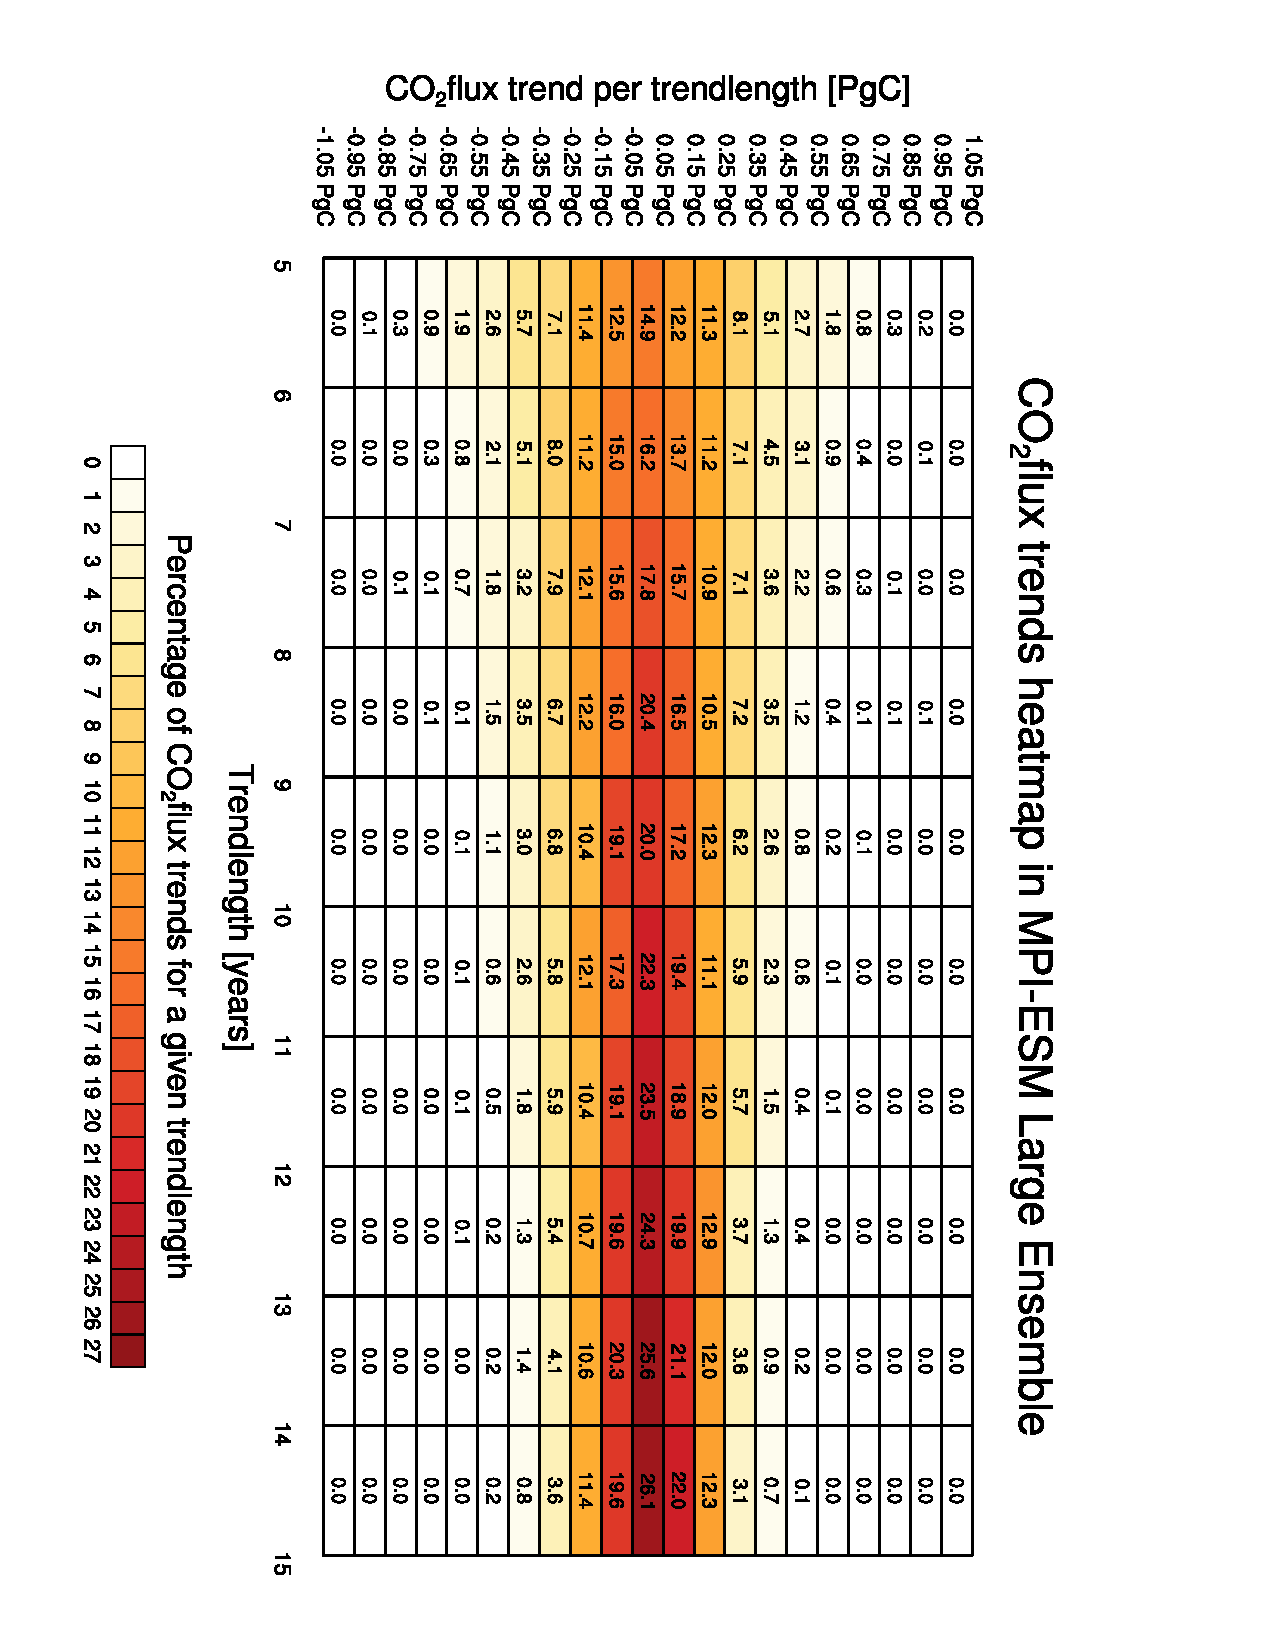
\includegraphics[scale=.64,angle=90,trim=1.3cm 1.3cm 5cm 1cm,clip]{heatmap_de-ens-trended.pdf} % from gfx folder
\caption{Southern Ocean carbon sink trends per trendlength; (above) normal; (below) detrended from ensmean trend}
	\label{fig:heatmap}
\end{figure}


\end{document}




















